\documentclass[10pt,compress,t,notes=noshow, xcolor=table]{beamer}


% graphicx and color are loaded via lmu-lecture.sty
% maxwidth is the original width if it is less than linewidth
% otherwise use linewidth (to make sure the graphics do not exceed the margin)
% TODO: Remove once cleared to be superfluous
% \makeatletter
% \def\maxwidth{ %
%   \ifdim\Gin@nat@width>\linewidth
%     \linewidth
%   \else
%     \Gin@nat@width
%   \fi
% }
% \makeatother

% ---------------------------------%
% latex-math dependencies, do not remove:
% - mathtools
% - bm
% - siunitx
% - dsfont
% - xspace
% ---------------------------------%

%--------------------------------------------------------%
%       Language, encoding, typography
%--------------------------------------------------------%

\usepackage[english]{babel}
\usepackage[utf8]{inputenc} % Enables inputting UTF-8 symbols
% Standard AMS suite (loaded via lmu-lecture.sty)

% Font for double-stroke / blackboard letters for sets of numbers (N, R, ...)
% Distribution name is "doublestroke"
% According to https://mirror.physik.tu-berlin.de/pub/CTAN/fonts/doublestroke/dsdoc.pdf
% the "bbm" package does a similar thing and may be superfluous.
% Required for latex-math
\usepackage{dsfont}

% bbm – "Blackboard-style" cm fonts (https://www.ctan.org/pkg/bbm)
% Used to be in common.tex, loaded directly after this file
% Maybe superfluous given dsfont is loaded
% TODO: Check if really unused?
% \usepackage{bbm}

% bm – Access bold symbols in maths mode - https://ctan.org/pkg/bm
% Required for latex-math, preferred over \boldsymbol
% https://tex.stackexchange.com/questions/3238/bm-package-versus-boldsymbol
\usepackage{bm}

% pifont – Access to PostScript standard Symbol and Dingbats fonts
% Used for \newcommand{\xmark}{\ding{55}, which is never used
% aside from lecture_advml/attic/xx-automl/slides.Rnw
% \usepackage{pifont}

% Quotes (inline and display), provdes \enquote
% https://ctan.org/pkg/csquotes
\usepackage{csquotes}

% Adds arg to enumerate env, technically superseded by enumitem according
% to https://ctan.org/pkg/enumerate
% Replace with https://ctan.org/pkg/enumitem ?
% Even better: enumitem is not really compatible with beamer and breaks all sorts of things
% particularly the enumerate environment. The enumerate package also just isn't required
% from what I can tell so... don't re-add it I guess?
% \usepackage{enumerate}

% Line spacing - provides \singlespacing \doublespacing \onehalfspacing
% https://ctan.org/pkg/setspace
% \usepackage{setspace}

% mathtools – Mathematical tools to use with amsmath
% https://ctan.org/pkg/mathtools?lang=en
% latex-math dependency according to latex-math repo
\usepackage{mathtools}

% Maybe not great to use this https://tex.stackexchange.com/a/197/19093
% Use align instead -- TODO: Global search & replace to check, eqnarray is used a lot
% $ rg -f -u "\begin{eqnarray" -l | grep -v attic | awk -F '/' '{print $1}' | sort | uniq -c
%   13 lecture_advml
%   14 lecture_i2ml
%    2 lecture_iml
%   27 lecture_optimization
%   45 lecture_sl
\usepackage{eqnarray}
% For shaded regions / boxes
% Used sometimes in optim
% https://www.ctan.org/pkg/framed
\usepackage{framed}

%--------------------------------------------------------%
%       Cite button (version 2024-05)
%--------------------------------------------------------%

% Superseded by style/ref-buttons.sty, kept just in case these don't work out somehow.

% Note this requires biber to be in $PATH when running,
% telltale error in log would be e.g. Package biblatex Info: ... file 'authoryear.dbx' not found
% aside from obvious "biber: command not found" or similar.
% Tried moving this to lmu-lecture.sty but had issues I didn't quite understood,
% so it's here for now.

\usepackage{hyperref}

% Only try adding a references file if it exists, otherwise
% this would compile error when references.bib is not found
% NOTE: Bibliography packages (usebib, biblatex) are now loaded by ref-buttons.sty when needed
% This keeps all bibliography-related setup in one place

% Legacy \citelink command removed - superseded by ref-buttons.sty

%--------------------------------------------------------%
%       Displaying code and algorithms
%--------------------------------------------------------%

% Reimplements verbatim environments: https://ctan.org/pkg/verbatim
% verbatim used sed at least once in
% supervised-classification/slides-classification-tasks.tex
% Removed since code should not be put on slides anyway
% \usepackage{verbatim}

% Both used together for algorithm typesetting, see also overleaf: https://www.overleaf.com/learn/latex/Algorithms
% algorithmic env is also used, but part of the bundle:
%   "algpseudocode is part of the algorithmicx bundle, it gives you an improved version of algorithmic besides providing some other features"
% According to https://tex.stackexchange.com/questions/229355/algorithm-algorithmic-algorithmicx-algorithm2e-algpseudocode-confused
\usepackage{algorithm}
\usepackage{algpseudocode}

%--------------------------------------------------------%
%       Tables
%--------------------------------------------------------%

% multi-row table cells: https://www.namsu.de/Extra/pakete/Multirow.html
% Provides \multirow
% Used e.g. in evaluation/slides-evaluation-measures-classification.tex
\usepackage{multirow}

% colortbl: https://ctan.org/pkg/colortbl
% "The package allows rows and columns to be coloured, and even individual cells." well.
% Provides \columncolor and \rowcolor
% \rowcolor is used multiple times, e.g. in knn/slides-knn.tex
\usepackage{colortbl}

% long/multi-page tables: https://texdoc.org/serve/longtable.pdf/0
% Not used in slides
% \usepackage{longtable}

% pretty table env: https://ctan.org/pkg/booktabs
% Is used
% Defines \toprule
\usepackage{booktabs}

%--------------------------------------------------------%
%       Figures: Creating, placing, verbing
%--------------------------------------------------------%

% wrapfig - Wrapping text around figures https://de.overleaf.com/learn/latex/Wrapping_text_around_figures
% Provides wrapfigure environment -used in lecture_optimization
\usepackage{wrapfig}

% Sub figures in figures and tables
% https://ctan.org/pkg/subfig -- supersedes subfigure package
% Provides \subfigure
% \subfigure not used in slides but slides-tuning-practical.pdf errors without this pkg, error due to \captionsetup undefined
\usepackage{subfig}

% Actually it's pronounced PGF https://en.wikibooks.org/wiki/LaTeX/PGF/TikZ
\usepackage{tikz}

% No idea what/why these settings are what they are but I assume they're there on purpose
\usetikzlibrary{shapes,arrows,automata,positioning,calc,chains,trees, shadows}
\tikzset{
  %Define standard arrow tip
  >=stealth',
  %Define style for boxes
  punkt/.style={
    rectangle,
    rounded corners,
    draw=black, very thick,
    text width=6.5em,
    minimum height=2em,
    text centered},
  % Define arrow style
  pil/.style={
    ->,
    thick,
    shorten <=2pt,
    shorten >=2pt,}
}

%--------------------------------------------------------%
%       Beamer setup and custom macros & environments
%--------------------------------------------------------%

% Main sty file for beamer setup (layout, style, lecture page numbering, etc.)
% For long-term maintenance, this may me refactored into a more modular set of .sty files
\usepackage{../../style/lmu-lecture}
% Custom itemize wrappers, itemizeS, itemizeL, etc
\usepackage{../../style/customitemize}
% Custom framei environment, uses custom itemize!
\usepackage{../../style/framei}
% Custom frame2 environment, allows specifying font size for all content
\usepackage{../../style/frame2}
% Column layout macros
\usepackage{../../style/splitV}
% \image and derivatives
\usepackage{../../style/image}
% New generation of reference button macros
\usepackage{../../style/ref-buttons}

% Used regularly
\let\code=\texttt

% Not sure what/why this does
\setkeys{Gin}{width=0.9\textwidth}

% -- knitr leftovers --
% These may be used by knitr/R Markdown workflows in other lectures
\makeatletter
\def\maxwidth{ %
  \ifdim\Gin@nat@width>\linewidth
    \linewidth
  \else
    \Gin@nat@width
  \fi
}
\makeatother

% Define colors for syntax highlighting (may be used by knitr)
\definecolor{fgcolor}{rgb}{0.345, 0.345, 0.345}
\definecolor{shadecolor}{rgb}{.97, .97, .97}

% knitr code output environment
\newenvironment{knitrout}{}{}


% Can't find a reason why common.tex is not just part of this file?
% This file is included in slides and exercises

% Rarely used fontstyle for R packages, used only in 
% - forests/slides-forests-benchmark.tex
% - exercises/single-exercises/methods_l_1.Rnw
% - slides/cart/attic/slides_extra_trees.Rnw
\newcommand{\pkg}[1]{{\fontseries{b}\selectfont #1}}

% Spacing helpers, used often (mostly in exercises for \dlz)
\newcommand{\lz}{\vspace{0.5cm}} % vertical space (used often in slides)
\newcommand{\dlz}{\vspace{1cm}}  % double vertical space (used often in exercises, never in slides)
\newcommand{\oneliner}[1] % Oneliner for important statements, used e.g. in iml, algods
{\begin{block}{}\begin{center}\begin{Large}#1\end{Large}\end{center}\end{block}}

% Don't know if this is used or needed, remove?
% textcolor that works in mathmode
% https://tex.stackexchange.com/a/261480
% Used e.g. in forests/slides-forests-bagging.tex
% [...] \textcolor{blue}{\tfrac{1}{M}\sum^M_{m} [...]
% \makeatletter
% \renewcommand*{\@textcolor}[3]{%
%   \protect\leavevmode
%   \begingroup
%     \color#1{#2}#3%
%   \endgroup
% }
% \makeatother


% math spaces
\ifdefined\N                                                                
\renewcommand{\N}{\mathds{N}} % N, naturals
\else \newcommand{\N}{\mathds{N}} \fi 
\newcommand{\Z}{\mathds{Z}} % Z, integers
\newcommand{\Q}{\mathds{Q}} % Q, rationals
\newcommand{\R}{\mathds{R}} % R, reals
\ifdefined\C 
  \renewcommand{\C}{\mathds{C}} % C, complex
\else \newcommand{\C}{\mathds{C}} \fi
\newcommand{\continuous}{\mathcal{C}} % C, space of continuous functions
\newcommand{\M}{\mathcal{M}} % machine numbers
\newcommand{\epsm}{\epsilon_m} % maximum error

% counting / finite sets
\newcommand{\setzo}{\{0, 1\}} % set 0, 1
\newcommand{\setmp}{\{-1, +1\}} % set -1, 1
\newcommand{\unitint}{[0, 1]} % unit interval

% basic math stuff
\newcommand{\xt}{\tilde x} % x tilde
\newcommand{\argmax}{\operatorname{arg\,max}} % argmax
\newcommand{\argmin}{\operatorname{arg\,min}} % argmin
\newcommand{\argopt}{\operatorname{arg\,opt}} % argopt
\newcommand{\argminlim}{\mathop{\mathrm{arg\,min}}\limits} % argmax with limits
\newcommand{\argmaxlim}{\mathop{\mathrm{arg\,max}}\limits} % argmin with limits  
\newcommand{\argoptlim}{\mathop{\mathrm{arg\,opt}}\limits} % argmin with limits  
\newcommand{\sign}{\operatorname{sign}} % sign, signum
\newcommand{\I}{\mathbb{I}} % I, indicator
\newcommand{\order}{\mathcal{O}} % O, order
\newcommand{\pd}[2]{\frac{\partial{#1}}{\partial #2}} % partial derivative
\newcommand{\floorlr}[1]{\left\lfloor #1 \right\rfloor} % floor
\newcommand{\ceillr}[1]{\left\lceil #1 \right\rceil} % ceiling

% sums and products
\newcommand{\sumin}{\sum\limits_{i=1}^n} % summation from i=1 to n
\newcommand{\sumim}{\sum\limits_{i=1}^m} % summation from i=1 to m
\newcommand{\sumjn}{\sum\limits_{j=1}^n} % summation from j=1 to p
\newcommand{\sumjp}{\sum\limits_{j=1}^p} % summation from j=1 to p
\newcommand{\sumik}{\sum\limits_{i=1}^k} % summation from i=1 to k
\newcommand{\sumkg}{\sum\limits_{k=1}^g} % summation from k=1 to g
\newcommand{\sumjg}{\sum\limits_{j=1}^g} % summation from j=1 to g
\newcommand{\meanin}{\frac{1}{n} \sum\limits_{i=1}^n} % mean from i=1 to n
\newcommand{\meankg}{\frac{1}{g} \sum\limits_{k=1}^g} % mean from k=1 to g
\newcommand{\prodin}{\prod\limits_{i=1}^n} % product from i=1 to n
\newcommand{\prodkg}{\prod\limits_{k=1}^g} % product from k=1 to g
\newcommand{\prodjp}{\prod\limits_{j=1}^p} % product from j=1 to p

% linear algebra
\newcommand{\one}{\boldsymbol{1}} % 1, unitvector
\newcommand{\zero}{\mathbf{0}} % 0-vector
\newcommand{\id}{\boldsymbol{I}} % I, identity
\newcommand{\diag}{\operatorname{diag}} % diag, diagonal
\newcommand{\trace}{\operatorname{tr}} % tr, trace
\newcommand{\spn}{\operatorname{span}} % span
\newcommand{\scp}[2]{\left\langle #1, #2 \right\rangle} % <.,.>, scalarproduct
\newcommand{\mat}[1]{\begin{pmatrix} #1 \end{pmatrix}} % short pmatrix command
\newcommand{\Amat}{\mathbf{A}} % matrix A
\newcommand{\Deltab}{\mathbf{\Delta}} % error term for vectors

% basic probability + stats
\renewcommand{\P}{\mathds{P}} % P, probability
\newcommand{\E}{\mathds{E}} % E, expectation
\newcommand{\var}{\mathsf{Var}} % Var, variance
\newcommand{\cov}{\mathsf{Cov}} % Cov, covariance
\newcommand{\corr}{\mathsf{Corr}} % Corr, correlation
\newcommand{\normal}{\mathcal{N}} % N of the normal distribution
\newcommand{\iid}{\overset{i.i.d}{\sim}} % dist with i.i.d superscript
\newcommand{\distas}[1]{\overset{#1}{\sim}} % ... is distributed as ...
% machine learning
\newcommand{\Xspace}{\mathcal{X}} % X, input space
\newcommand{\Yspace}{\mathcal{Y}} % Y, output space
\newcommand{\Zspace}{\mathcal{Z}} % Z, space of sampled datapoints
\newcommand{\nset}{\{1, \ldots, n\}} % set from 1 to n
\newcommand{\pset}{\{1, \ldots, p\}} % set from 1 to p
\newcommand{\gset}{\{1, \ldots, g\}} % set from 1 to g
\newcommand{\Pxy}{\mathbb{P}_{xy}} % P_xy
\newcommand{\Exy}{\mathbb{E}_{xy}} % E_xy: Expectation over random variables xy
\newcommand{\xv}{\mathbf{x}} % vector x (bold)
\newcommand{\xtil}{\tilde{\mathbf{x}}} % vector x-tilde (bold)
\newcommand{\yv}{\mathbf{y}} % vector y (bold)
\newcommand{\xy}{(\xv, y)} % observation (x, y)
\newcommand{\xvec}{\left(x_1, \ldots, x_p\right)^\top} % (x1, ..., xp)
\newcommand{\Xmat}{\mathbf{X}} % Design matrix
\newcommand{\allDatasets}{\mathds{D}} % The set of all datasets
\newcommand{\allDatasetsn}{\mathds{D}_n}  % The set of all datasets of size n
\newcommand{\D}{\mathcal{D}} % D, data
\newcommand{\Dn}{\D_n} % D_n, data of size n
\newcommand{\Dtrain}{\mathcal{D}_{\text{train}}} % D_train, training set
\newcommand{\Dtest}{\mathcal{D}_{\text{test}}} % D_test, test set
\newcommand{\xyi}[1][i]{\left(\xv^{(#1)}, y^{(#1)}\right)} % (x^i, y^i), i-th observation
\newcommand{\Dset}{\left( \xyi[1], \ldots, \xyi[n]\right)} % {(x1,y1)), ..., (xn,yn)}, data
\newcommand{\defAllDatasetsn}{(\Xspace \times \Yspace)^n} % Def. of the set of all datasets of size n
\newcommand{\defAllDatasets}{\bigcup_{n \in \N}(\Xspace \times \Yspace)^n} % Def. of the set of all datasets
\newcommand{\xdat}{\left\{ \xv^{(1)}, \ldots, \xv^{(n)}\right\}} % {x1, ..., xn}, input data
\newcommand{\ydat}{\left\{ \yv^{(1)}, \ldots, \yv^{(n)}\right\}} % {y1, ..., yn}, input data
\newcommand{\yvec}{\left(y^{(1)}, \hdots, y^{(n)}\right)^\top} % (y1, ..., yn), vector of outcomes
\newcommand{\greekxi}{\xi} % Greek letter xi
\renewcommand{\xi}[1][i]{\xv^{(#1)}} % x^i, i-th observed value of x
\newcommand{\yi}[1][i]{y^{(#1)}} % y^i, i-th observed value of y
\newcommand{\xivec}{\left(x^{(i)}_1, \ldots, x^{(i)}_p\right)^\top} % (x1^i, ..., xp^i), i-th observation vector
\newcommand{\xj}{\xv_j} % x_j, j-th feature
\newcommand{\xjvec}{\left(x^{(1)}_j, \ldots, x^{(n)}_j\right)^\top} % (x^1_j, ..., x^n_j), j-th feature vector
\newcommand{\phiv}{\mathbf{\phi}} % Basis transformation function phi
\newcommand{\phixi}{\mathbf{\phi}^{(i)}} % Basis transformation of xi: phi^i := phi(xi)

%%%%%% ml - models general
\newcommand{\lamv}{\bm{\lambda}} % lambda vector, hyperconfiguration vector
\newcommand{\Lam}{\Lambda}	 % Lambda, space of all hpos
% Inducer / Inducing algorithm
\newcommand{\preimageInducer}{\left(\defAllDatasets\right)\times\Lam} % Set of all datasets times the hyperparameter space
\newcommand{\preimageInducerShort}{\allDatasets\times\Lam} % Set of all datasets times the hyperparameter space
% Inducer / Inducing algorithm
\newcommand{\ind}{\mathcal{I}} % Inducer, inducing algorithm, learning algorithm

% continuous prediction function f
\newcommand{\ftrue}{f_{\text{true}}}  % True underlying function (if a statistical model is assumed)
\newcommand{\ftruex}{\ftrue(\xv)} % True underlying function (if a statistical model is assumed)
\newcommand{\fx}{f(\xv)} % f(x), continuous prediction function
\newcommand{\fdomains}{f: \Xspace \rightarrow \R^g} % f with domain and co-domain
\newcommand{\Hspace}{\mathcal{H}} % hypothesis space where f is from
\newcommand{\Hall}{\mathcal{H}_{\text{all}}} % unrestricted hypothesis space
\newcommand{\fbayes}{f^{\ast}} % Bayes-optimal model
\newcommand{\fxbayes}{f^{\ast}(\xv)} % Bayes-optimal model
\newcommand{\fkx}[1][k]{f_{#1}(\xv)} % f_j(x), discriminant component function
\newcommand{\fhspace}{\hat f_{\Hspace}} % fhat_H
\newcommand{\fh}{\hat{f}} % f hat, estimated prediction function
\newcommand{\fxh}{\fh(\xv)} % fhat(x)
\newcommand{\fxt}{f(\xv ~|~ \thetav)} % f(x | theta)
\newcommand{\fxi}{f\left(\xv^{(i)}\right)} % f(x^(i))
\newcommand{\fxih}{\hat{f}\left(\xv^{(i)}\right)} % f(x^(i))
\newcommand{\fxit}{f\big(\xv^{(i)} ~|~ \thetav\big)} % f(x^(i) | theta)
\newcommand{\fhD}{\fh_{\D}} % fhat_D, estimate of f based on D
\newcommand{\fhDtrain}{\fh_{\Dtrain}} % fhat_Dtrain, estimate of f based on D
\newcommand{\fhDnlam}{\fh_{\Dn, \lamv}} %model learned on Dn with hp lambda
\newcommand{\fhDlam}{\fh_{\D, \lamv}} %model learned on D with hp lambda
\newcommand{\fhDnlams}{\fh_{\Dn, \lamv^\ast}} %model learned on Dn with optimal hp lambda
\newcommand{\fhDlams}{\fh_{\D, \lamv^\ast}} %model learned on D with optimal hp lambda

% discrete prediction function h
\newcommand{\hx}{h(\xv)} % h(x), discrete prediction function
\newcommand{\hh}{\hat{h}} % h hat
\newcommand{\hxh}{\hat{h}(\xv)} % hhat(x)
\newcommand{\hxt}{h(\xv | \thetav)} % h(x | theta)
\newcommand{\hxi}{h\left(\xi\right)} % h(x^(i))
\newcommand{\hxit}{h\left(\xi ~|~ \thetav\right)} % h(x^(i) | theta)
\newcommand{\hbayes}{h^{\ast}} % Bayes-optimal classification model
\newcommand{\hxbayes}{h^{\ast}(\xv)} % Bayes-optimal classification model

% yhat
\newcommand{\yh}{\hat{y}} % yhat for prediction of target
\newcommand{\yih}{\hat{y}^{(i)}} % yhat^(i) for prediction of ith targiet
\newcommand{\resi}{\yi- \yih}

% theta
\newcommand{\thetah}{\hat{\theta}} % theta hat
\newcommand{\thetav}{\bm{\theta}} % theta vector
\newcommand{\thetavh}{\bm{\hat\theta}} % theta vector hat
\newcommand{\thetat}[1][t]{\thetav^{[#1]}} % theta^[t] in optimization
\newcommand{\thetatn}[1][t]{\thetav^{[#1 +1]}} % theta^[t+1] in optimization
\newcommand{\thetahDnlam}{\thetavh_{\Dn, \lamv}} %theta learned on Dn with hp lambda
\newcommand{\thetahDlam}{\thetavh_{\D, \lamv}} %theta learned on D with hp lambda
\newcommand{\mint}{\min_{\thetav \in \Theta}} % min problem theta
\newcommand{\argmint}{\argmin_{\thetav \in \Theta}} % argmin theta

% densities + probabilities
% pdf of x
\newcommand{\pdf}{p} % p
\newcommand{\pdfx}{p(\xv)} % p(x)
\newcommand{\pixt}{\pi(\xv~|~ \thetav)} % pi(x|theta), pdf of x given theta
\newcommand{\pixit}[1][i]{\pi\left(\xi[#1] ~|~ \thetav\right)} % pi(x^i|theta), pdf of x given theta
\newcommand{\pixii}[1][i]{\pi\left(\xi[#1]\right)} % pi(x^i), pdf of i-th x

% pdf of (x, y)
\newcommand{\pdfxy}{p(\xv,y)} % p(x, y)
\newcommand{\pdfxyt}{p(\xv, y ~|~ \thetav)} % p(x, y | theta)
\newcommand{\pdfxyit}{p\left(\xi, \yi ~|~ \thetav\right)} % p(x^(i), y^(i) | theta)

% pdf of x given y
\newcommand{\pdfxyk}[1][k]{p(\xv | y= #1)} % p(x | y = k)
\newcommand{\lpdfxyk}[1][k]{\log p(\xv | y= #1)} % log p(x | y = k)
\newcommand{\pdfxiyk}[1][k]{p\left(\xi | y= #1 \right)} % p(x^i | y = k)

% prior probabilities
\newcommand{\pik}[1][k]{\pi_{#1}} % pi_k, prior
\newcommand{\pih}{\hat{\pi}} % pi hat, estimated prior (binary classification)
\newcommand{\pikh}[1][k]{\hat{\pi}_{#1}} % pi_k hat, estimated prior
\newcommand{\lpik}[1][k]{\log \pi_{#1}} % log pi_k, log of the prior
\newcommand{\pit}{\pi(\thetav)} % Prior probability of parameter theta

% posterior probabilities
\newcommand{\post}{\P(y = 1 ~|~ \xv)} % P(y = 1 | x), post. prob for y=1
\newcommand{\postk}[1][k]{\P(y = #1 ~|~ \xv)} % P(y = k | y), post. prob for y=k
\newcommand{\pidomains}{\pi: \Xspace \rightarrow \unitint} % pi with domain and co-domain
\newcommand{\pibayes}{\pi^{\ast}} % Bayes-optimal classification model
\newcommand{\pixbayes}{\pi^{\ast}(\xv)} % Bayes-optimal classification model
\newcommand{\piastxtil}{\pi^{\ast}(\xtil)} % Bayes-optimal classification model
\newcommand{\piastkxtil}{\pi^{\ast}_k(\xtil)} % Bayes-optimal classification model for k-th class
\newcommand{\pix}{\pi(\xv)} % pi(x), P(y = 1 | x)
\newcommand{\piv}{\bm{\pi}} % pi, bold, as vector
\newcommand{\pikx}[1][k]{\pi_{#1}(\xv)} % pi_k(x), P(y = k | x)
\newcommand{\pikxt}[1][k]{\pi_{#1}(\xv ~|~ \thetav)} % pi_k(x | theta), P(y = k | x, theta)
\newcommand{\pixh}{\hat \pi(\xv)} % pi(x) hat, P(y = 1 | x) hat
\newcommand{\pikxh}[1][k]{\hat \pi_{#1}(\xv)} % pi_k(x) hat, P(y = k | x) hat
\newcommand{\pixih}{\hat \pi(\xi)} % pi(x^(i)) with hat
\newcommand{\pikxih}[1][k]{\hat \pi_{#1}(\xi)} % pi_k(x^(i)) with hat
\newcommand{\pdfygxt}{p(y ~|~\xv, \thetav)} % p(y | x, theta)
\newcommand{\pdfyigxit}{p\left(\yi ~|~\xi, \thetav\right)} % p(y^i |x^i, theta)
\newcommand{\lpdfygxt}{\log \pdfygxt } % log p(y | x, theta)
\newcommand{\lpdfyigxit}{\log \pdfyigxit} % log p(y^i |x^i, theta)

% probabilistic
\newcommand{\bayesrulek}[1][k]{\frac{\P(\xv | y= #1) \P(y= #1)}{\P(\xv)}} % Bayes rule
\newcommand{\muv}{\bm{\mu}} % expectation vector of Gaussian
\newcommand{\muk}[1][k]{\bm{\mu_{#1}}} % mean vector of class-k Gaussian (discr analysis)
\newcommand{\mukh}[1][k]{\bm{\hat{\mu}_{#1}}} % estimated mean vector of class-k Gaussian (discr analysis)

% residual and margin
\newcommand{\rx}{r(\xv)} % residual 
\newcommand{\eps}{\epsilon} % residual, stochastic
\newcommand{\epsv}{\bm{\epsilon}} % residual, stochastic, as vector
\newcommand{\epsi}{\epsilon^{(i)}} % epsilon^i, residual, stochastic
\newcommand{\epsh}{\hat{\epsilon}} % residual, estimated
\newcommand{\epsvh}{\hat{\epsv}} % residual, estimated, vector
\newcommand{\yf}{y \fx} % y f(x), margin
\newcommand{\yfi}{\yi \fxi} % y^i f(x^i), margin
\newcommand{\Sigmah}{\hat \Sigma} % estimated covariance matrix
\newcommand{\Sigmahj}{\hat \Sigma_j} % estimated covariance matrix for the j-th class
\newcommand{\nux}{\nu(\xv)} % nu(x) = y * f(x)

% ml - loss, risk, likelihood
\newcommand{\Lyf}{L\left(y, f\right)} % L(y, f), loss function
% \newcommand{\Lypi}{L\left(y, \pi\right)} % L(y, pi), loss function
\newcommand{\Lxy}{L\left(y, \fx\right)} % L(y, f(x)), loss function
\newcommand{\Lxyi}{L\left(\yi, \fxi\right)} % loss of observation
\newcommand{\Lxyt}{L\left(y, \fxt\right)} % loss with f parameterized
\newcommand{\Lxyit}{L\left(\yi, \fxit\right)} % loss of observation with f parameterized
\newcommand{\Lxym}{L\left(\yi, f\left(\bm{\tilde{x}}^{(i)} ~|~ \thetav\right)\right)} % loss of observation with f parameterized
\newcommand{\Lpixy}{L\left(y, \pix\right)} % loss in classification
% \newcommand{\Lpiy}{L\left(y, \pi\right)} % loss in classification
\newcommand{\Lpiv}{L\left(y, \piv\right)} % loss in classification
\newcommand{\Lpixyi}{L\left(\yi, \pixii\right)} % loss of observation in classification
\newcommand{\Lpixyt}{L\left(y, \pixt\right)} % loss with pi parameterized
\newcommand{\Lpixyit}{L\left(\yi, \pixit\right)} % loss of observation with pi parameterized
% \newcommand{\Lhy}{L\left(y, h\right)} % L(y, h), loss function on discrete classes
\newcommand{\Lhxy}{L\left(y, \hx\right)} % L(y, h(x)), loss function on discrete classes
\newcommand{\Lr}{L\left(r\right)} % L(r), loss defined on residual (reg) / margin (classif)
\newcommand{\lone}{|y - \fx|} % L1 loss
\newcommand{\ltwo}{\left(y - \fx\right)^2} % L2 loss
\newcommand{\lbernoullimp}{\ln(1 + \exp(-y \cdot \fx))} % Bernoulli loss for -1, +1 encoding
\newcommand{\lbernoullizo}{- y \cdot \fx + \log(1 + \exp(\fx))} % Bernoulli loss for 0, 1 encoding
\newcommand{\lcrossent}{- y \log \left(\pix\right) - (1 - y) \log \left(1 - \pix\right)} % cross-entropy loss
\newcommand{\lbrier}{\left(\pix - y \right)^2} % Brier score
\newcommand{\risk}{\mathcal{R}} % R, risk
\newcommand{\riskbayes}{\mathcal{R}^\ast}
\newcommand{\riskf}{\risk(f)} % R(f), risk
\newcommand{\riskdef}{\E_{y|\xv}\left(\Lxy \right)} % risk def (expected loss)
\newcommand{\riskt}{\mathcal{R}(\thetav)} % R(theta), risk
\newcommand{\riske}{\mathcal{R}_{\text{emp}}} % R_emp, empirical risk w/o factor 1 / n
\newcommand{\riskeb}{\bar{\mathcal{R}}_{\text{emp}}} % R_emp, empirical risk w/ factor 1 / n
\newcommand{\riskef}{\riske(f)} % R_emp(f)
\newcommand{\risket}{\mathcal{R}_{\text{emp}}(\thetav)} % R_emp(theta)
\newcommand{\riskr}{\mathcal{R}_{\text{reg}}} % R_reg, regularized risk
\newcommand{\riskrt}{\mathcal{R}_{\text{reg}}(\thetav)} % R_reg(theta)
\newcommand{\riskrf}{\riskr(f)} % R_reg(f)
\newcommand{\riskrth}{\hat{\mathcal{R}}_{\text{reg}}(\thetav)} % hat R_reg(theta)
\newcommand{\risketh}{\hat{\mathcal{R}}_{\text{emp}}(\thetav)} % hat R_emp(theta)
\newcommand{\LL}{\mathcal{L}} % L, likelihood
\newcommand{\LLt}{\mathcal{L}(\thetav)} % L(theta), likelihood
\newcommand{\LLtx}{\mathcal{L}(\thetav | \xv)} % L(theta|x), likelihood
\newcommand{\logl}{\ell} % l, log-likelihood
\newcommand{\loglt}{\logl(\thetav)} % l(theta), log-likelihood
\newcommand{\logltx}{\logl(\thetav | \xv)} % l(theta|x), log-likelihood
\newcommand{\errtrain}{\text{err}_{\text{train}}} % training error
\newcommand{\errtest}{\text{err}_{\text{test}}} % test error
\newcommand{\errexp}{\overline{\text{err}_{\text{test}}}} % avg training error

% lm
\newcommand{\thx}{\thetav^\top \xv} % linear model
\newcommand{\olsest}{(\Xmat^\top \Xmat)^{-1} \Xmat^\top \yv} % OLS estimator in LM



\usepackage{etoolbox}
\makeatletter
\newlength{\parboxtodim}
\patchcmd{\@iiiparbox}
  {\hsize}
  {\ifx\relax#2\else\setlength{\parboxtodim}{#2}\fi\hsize}
  {}{}
\makeatother

\setbeamersize{text margin left=0.3cm,text margin right=0.3cm}

\begin{document}

\title{Applied Machine Learning}

\titlemeta{
The Data Science Lifecycle
}{
Main phases
}{
figure_man/DSLifecycle1
}{
  \item Know phases of data science lifecycle
  \item Identify essential concepts, tools, and methods for each phase
}

% \begin{frame}[plain]
% \titlepage
% \end{frame}


% \begin{frame}[plain]{}
% \phantomsection\label{section}
% \end{frame}

% \section{The Data Science Lifecycle}\label{the-data-science-lifecycle}

% \begin{frame}{Learning Objectives}
% By the end of this session, you should be able to:
% \begin{itemize}
%   \item Describe key phases of the data science lifecycle
%   \item Identify essential concepts, tools, and methods for each phase
%   \item Plan an end-to-end ML workflow with attention to constraints and dependencies
% \end{itemize}

% \end{frame}

\begin{frame}{The Data Science Lifecycle \furtherreading{CRISP}}
\phantomsection\label{the-data-science-lifecycle-1}
\textbf{Lifecycle Management}: Process of managing a (product) lifecycle from inception, through engineering, design and manufacturing to deployment and eventual disposal.

\textbf{CRISP-DM (Cross-Industry Standard Process for Data Mining)}:
A widely used framework that formalizes the iterative process of turning data into knowledge. 

%https://docs.google.com/presentation/d/1RCourH6lXL6sycgT6HbIXWb7rnQvA5HJ/edit?slide=id.p1#slide=id.p1
% \begin{figure}[h]
% 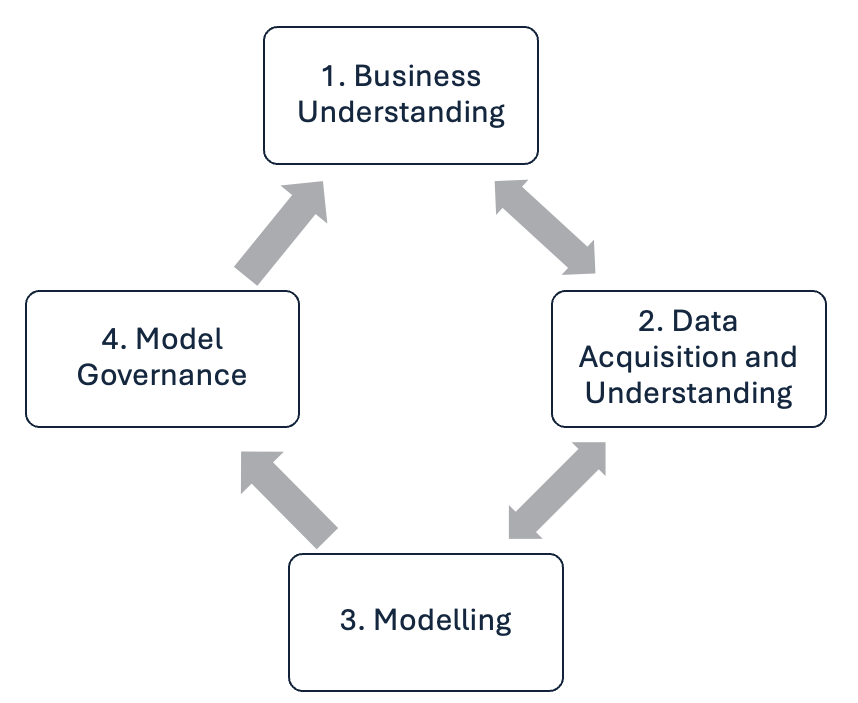
\includegraphics[width=7cm]{figure_man/DSLifecycle1.png}
% \end{figure}

% \end{frame}

% \begin{frame}{The Data Science Lifecycle}
% \phantomsection\label{the-data-science-lifecycle-1}

%https://docs.google.com/presentation/d/1RCourH6lXL6sycgT6HbIXWb7rnQvA5HJ/edit?slide=id.p1#slide=id.p1
\begin{figure}[h]
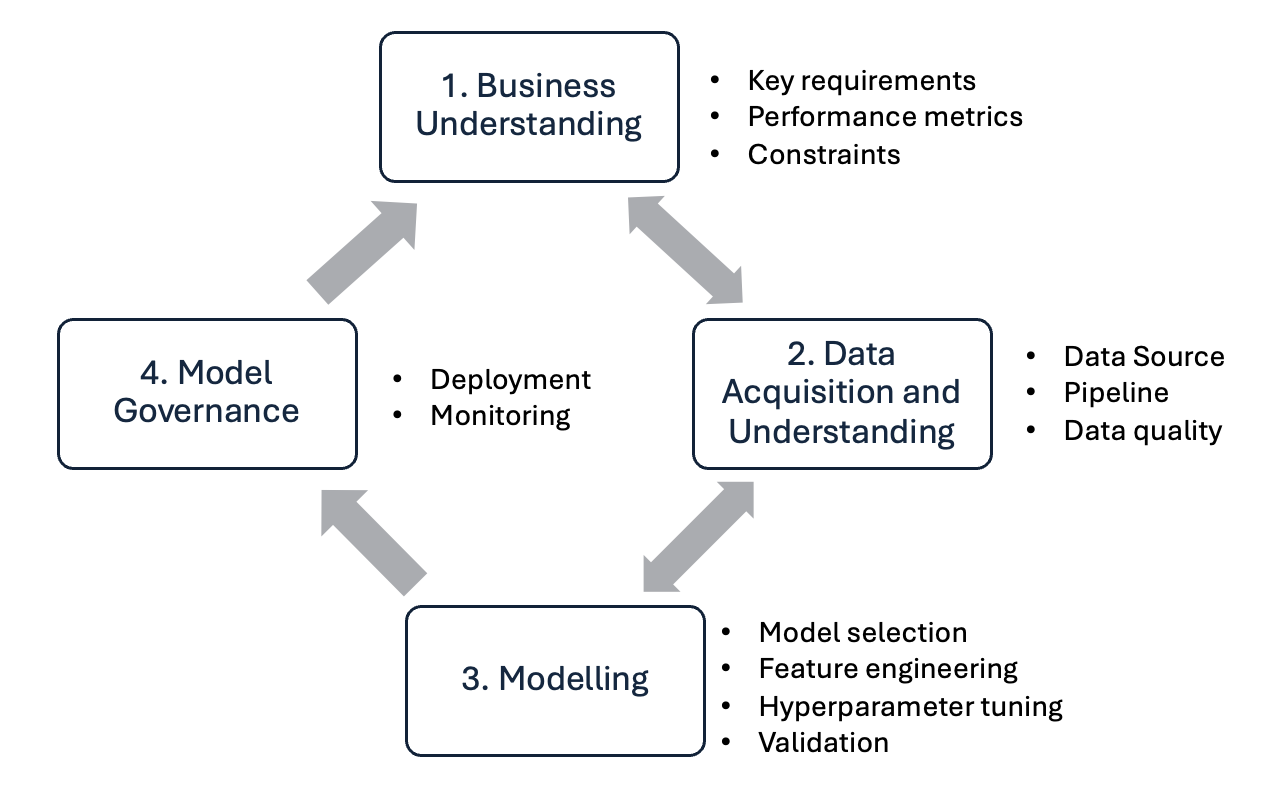
\includegraphics[width=9cm]{figure_man/DSLifecycle2.png}
\end{figure}

\end{frame}


\section{1. Business Understanding}\label{business-understanding-1}

\begin{frame}{Overview Business Understanding}
%https://docs.google.com/presentation/d/1RCourH6lXL6sycgT6HbIXWb7rnQvA5HJ/edit?slide=id.p1#slide=id.p1
\begin{figure}[h]
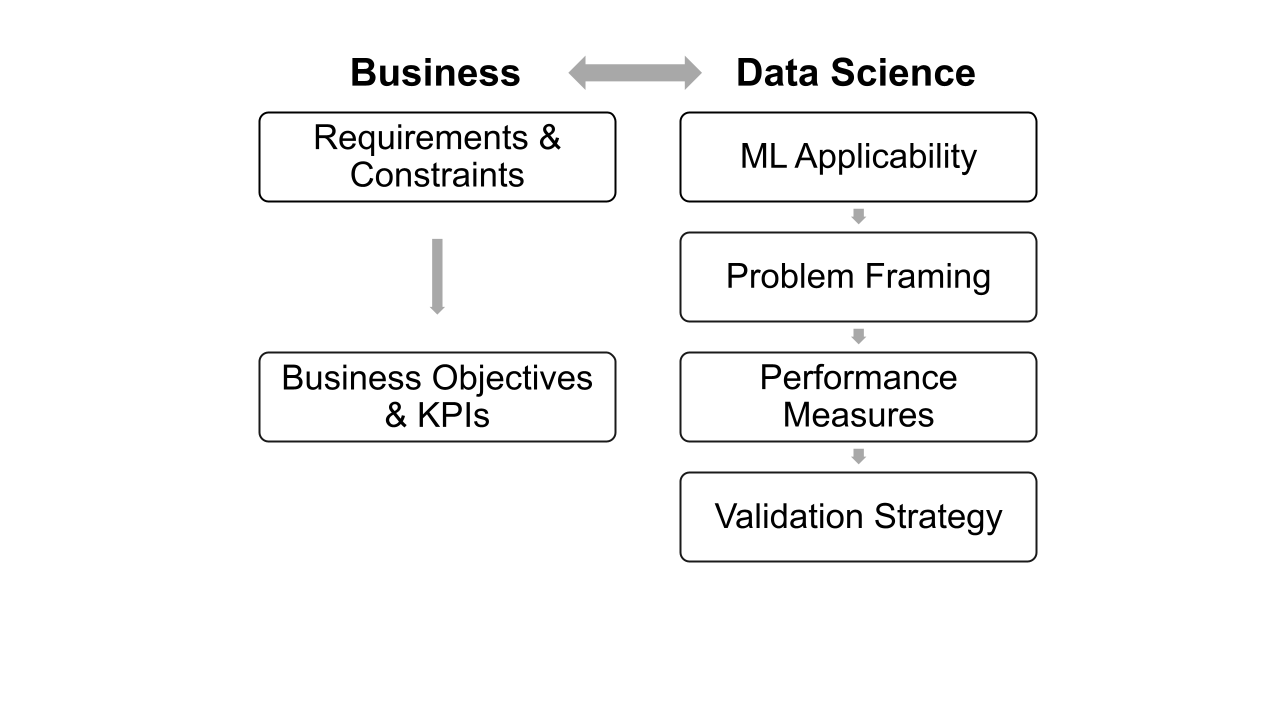
\includegraphics[width=\textwidth]{figure_man/BusinessUnderstandingOverview.png}
\end{figure}
\end{frame}

\begin{frame}{Requirements \& Constraints}
\phantomsection\label{requirements-analysis}
\textbf{Key question}: What is the end goal of the project?
\begin{itemize}
% \tightlist
\item
  Define the intended \textbf{output}:
  \begin{itemize}
  % \tightlist
      \item Report, dashboard, or interactive tool?
      \item Scalable pipeline for production use?
  \end{itemize}
\pause
\item Identify constraints% (--> Summarized in \textbf{Service Level Agreements})
    \begin{itemize}
      % \tightlist
      \item
        Ethical: Avoid sensitive data use (e.g., address may proxy ethnicity)
      \item
        Legal: Exclude protected attributes (e.g., gender in automated hiring)  %in automated decisions (e.g., job applications).
      \item
        Reproducibility: Ensure the analysis is fully reproducible in a single step
      \item
        Explainability: All model decisions must be explainable to the user
        \item Prediction Latency: Real-time predictions required
        \item Model Size: Stay within specified memory constraints
      \end{itemize}
\end{itemize}
\end{frame}

\begin{frame}{Requirements \& Constraints}
\phantomsection\label{requirements-ml-framing}

\textbf{1. ML Applicability: Is ML justified?}
\begin{itemize}
  % \tightlist
  \item Explore non-ML baselines first (rules, heuristics, simple analytics)
  \item Use ML only if it adds clear value over simpler/existing alternatives
\end{itemize}
\pause
\textbf{2. Problem Framing: How to frame the task?}
\begin{itemize}
  % \tightlist
  \item \emph{Imbalanced data:} classification vs.\ anomaly detection?
  \item \emph{Pred. maintenance:} failure probability (classif.) vs.\ remaining lifetime (regr.)?
  \item Select the ML task that aligns with your KPI and data characteristics
\end{itemize}

\centering
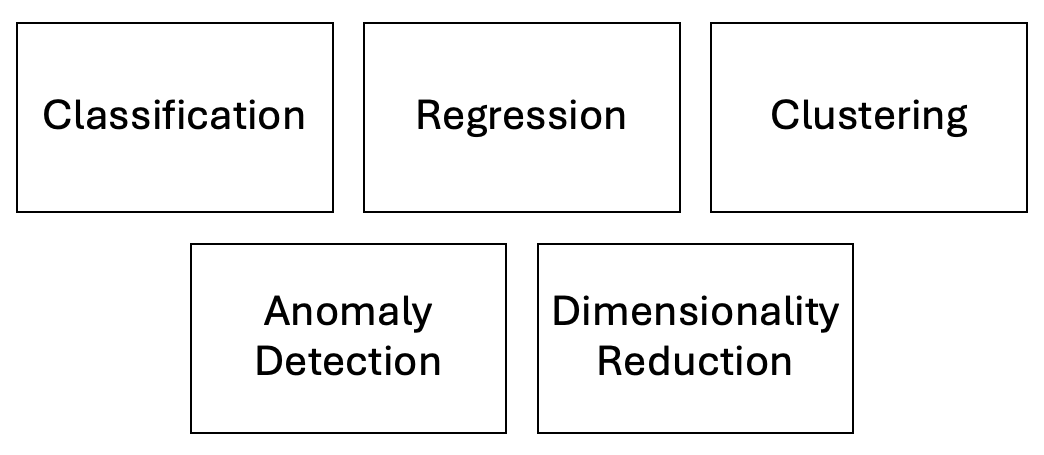
\includegraphics[width=0.6\textwidth]{figure_man/MLTasks.png}
\end{frame}

% \begin{frame}{Requirements Analysis: ML Application}
% \phantomsection\label{non-ml-baseline}
% \textbf{Key question}: Is ML necessary or is a simpler non-ML baseline sufficient?
% \begin{itemize}
% \tightlist
%   \item Consider simpler alternatives first
%   \item Evaluate current rule-based or heuristic systems
%   \item ML is justified when patterns are too complex or dynamic for rules
% \end{itemize}
% \end{frame}

% \begin{frame}{Requirements Analysis: Problem Frame}
% \phantomsection\label{choosing-the-right-problem-frame}
% \textbf{Key question}: Is it classification, regression or something else?
% \begin{itemize}
% \tightlist
% \item
%   A highly imbalanced problem: Frame it as classification, or anomaly
%   detection?
% \item
%   Predictive maintenance: Frame it as classification (probability of
%   failure), or regression (expected remaining lifetime)?
% \item
%   The answer is not clear, but depends on your application. It's
%   important to think about these problems!
% \end{itemize}
% ML-tasks you can select from:
% %https://docs.google.com/presentation/d/1RCourH6lXL6sycgT6HbIXWb7rnQvA5HJ/edit?slide=id.p1#slide=id.p1
% \begin{figure}[h]
% 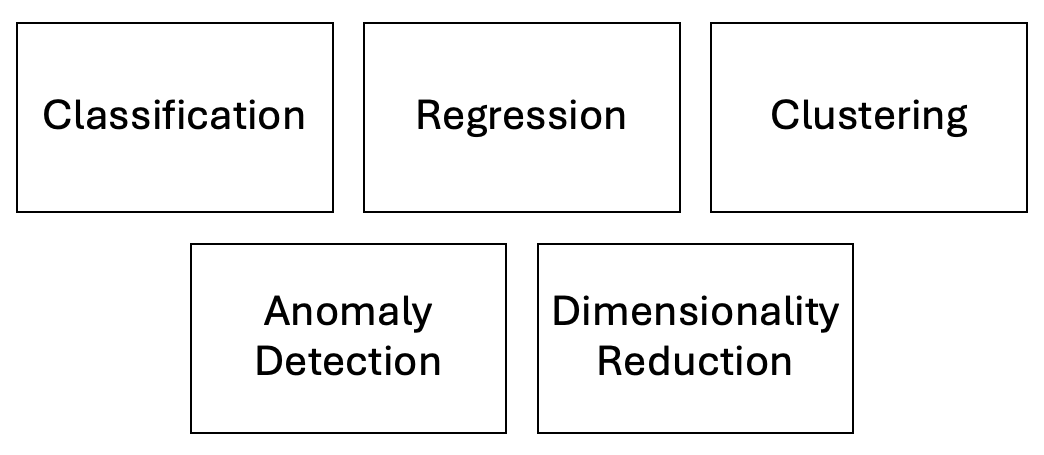
\includegraphics[width=7cm]{figure_man/MLTasks.png}
% \end{figure}
% \end{frame}


% \begin{frame}{KPIs and Business Objectives}
% \phantomsection\label{translating-kpis-into-performance-measures}
% \textbf{KPI}: Key Performance Indicator

% \textbf{Key question}: How does the business side measure success/ performance of the ML solution? How can we translate this to a ML performance measure?

% \begin{itemize}
% \tightlist
% \item
%   Spam detection:

% \begin{itemize}
%   \tightlist
%   \item
%     \emph{Not} OK to misclassify a job application as spam (positive
%     class)
%   \item
%     A spam mail in your inbox once in a while is no problem\\
%     \(\rightarrow\) \emph{minimize the false positive rate},
%     i.e.~maximize precision
%   \end{itemize}
% \item
%   Airport security:

%   \begin{itemize}
%   \tightlist
%   \item
%     \emph{Not} OK to misclassify a weapon (positive class) as laptop
%   \item
%     A false alarm once in a while is no problem\\
%     \(\rightarrow\) \emph{minimize the false negative rate},
%     i.e.~maximize recall
%   \end{itemize}
% \end{itemize}

% \end{frame}

% \begin{frame}{Multiple Objectives}
% \phantomsection\label{multiple-objectives}
% \textbf{Key question}: How to optimize multiple objectives?
% \begin{itemize}
% \tightlist
% \item
%   What if a choice increases objective 1, but decreases objective 2? Is
%   it better?
% \item Maybe maximizing AUC leads to more model complexity and less explainability
% \item
%   There are two common ways to deal with multiple objectives:

%   \begin{itemize}
%   \tightlist
%   \item
%     \textbf{Scalarization} in a \emph{compound measure}:
%     \(obj_1 * obj_2\)
%   \item
%     \textbf{Multi-objective Analysis} %TODO add link for further reading
%   \end{itemize}
% \end{itemize}
% \end{frame}



% \begin{frame}{Performance Measures}
% \phantomsection\label{performance-measures}

% \textbf{Key question}: what performance measure suits best for your solution?

% \begin{itemize}
% \tightlist
%     \item \textbf{Precision and Recall}%: $Precision = \frac{TP}{TP+FP}$, $Recall = \frac{TP}{TP+FN}$
%     \item to capture the tradeoff \textbf{F1-score} $F1 = \frac{2*Recall*Precision}{Recall + Precision}$
%     \item \textbf{Accuracy}: %$Acc = \frac{TP+TN}{TP+TN+FP+FN}$
%     for highly imbalanced data, the accuracy
%   (percentage of correct predictions) is not a good measure
%   \item I.e. in an HIV test, where 99.9\% of the population is healthy, a senseless
%   test that predicts ``healthy'' \emph{all the time}, automatically has
%   an accuracy of 99.9\%
% \end{itemize}

% %https://docs.google.com/presentation/d/1RCourH6lXL6sycgT6HbIXWb7rnQvA5HJ/edit?slide=id.p1#slide=id.p1
% \begin{figure}[h]
% 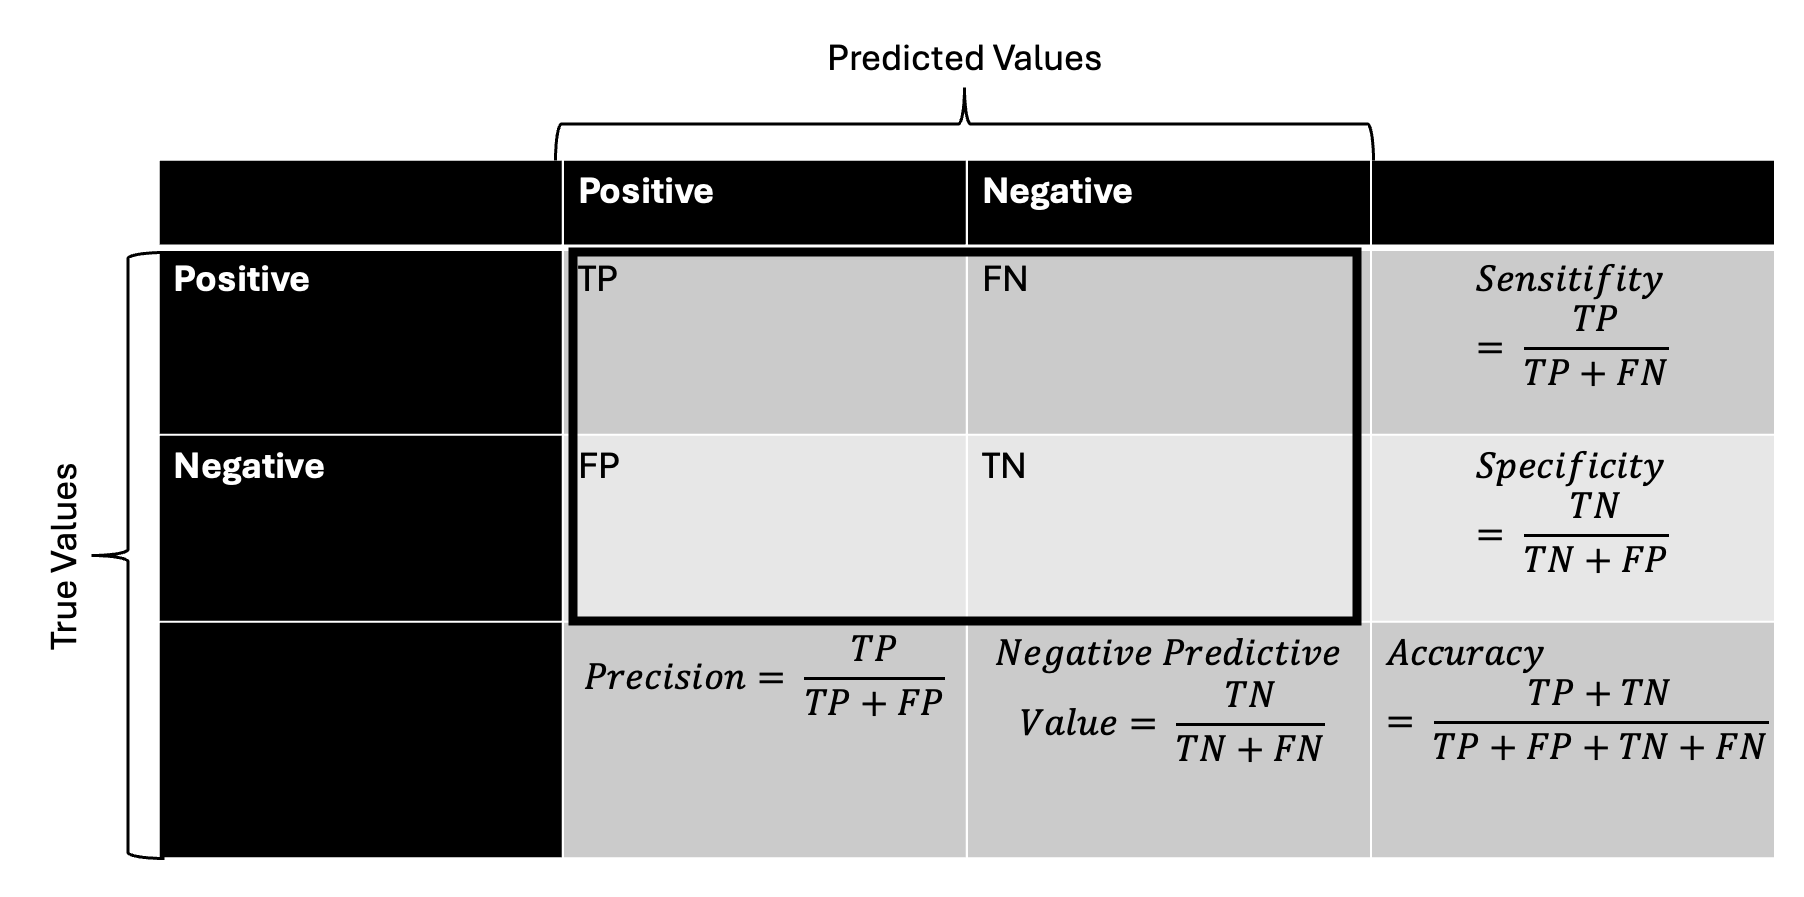
\includegraphics[width=0.72\textwidth]{figure_man/ConfusionMatrix.png}
% \end{figure}
% \end{frame}


\begin{frame}{Business Objectives: Performance Measures}
\phantomsection\label{kpi-metrics-slide}
\vspace{-0.5em}
\begin{itemize}
  % \tightlist
  %-----------------------------------------------------------
  \item<1-> \textbf{How to translate key performance indicators (KPIs) to metrics?}
\begin{itemize}
  % \tightlist
  \item \textbf{Spam detection}: Job application flagged as spam = unacceptable\\
      $\Rightarrow$ Occasional inbox spam is fine $\Rightarrow$ minimize FP $\Rightarrow$ maximize \textbf{precision}
  \item \textbf{Airport security}:  Weapon flagged as laptop = unacceptable\\
      $\Rightarrow$ Occasional false alarm is fine $\Rightarrow$ minimize FN $\Rightarrow$ maximize \textbf{recall}
\end{itemize}

\only<1>{
    \begin{center}
        
    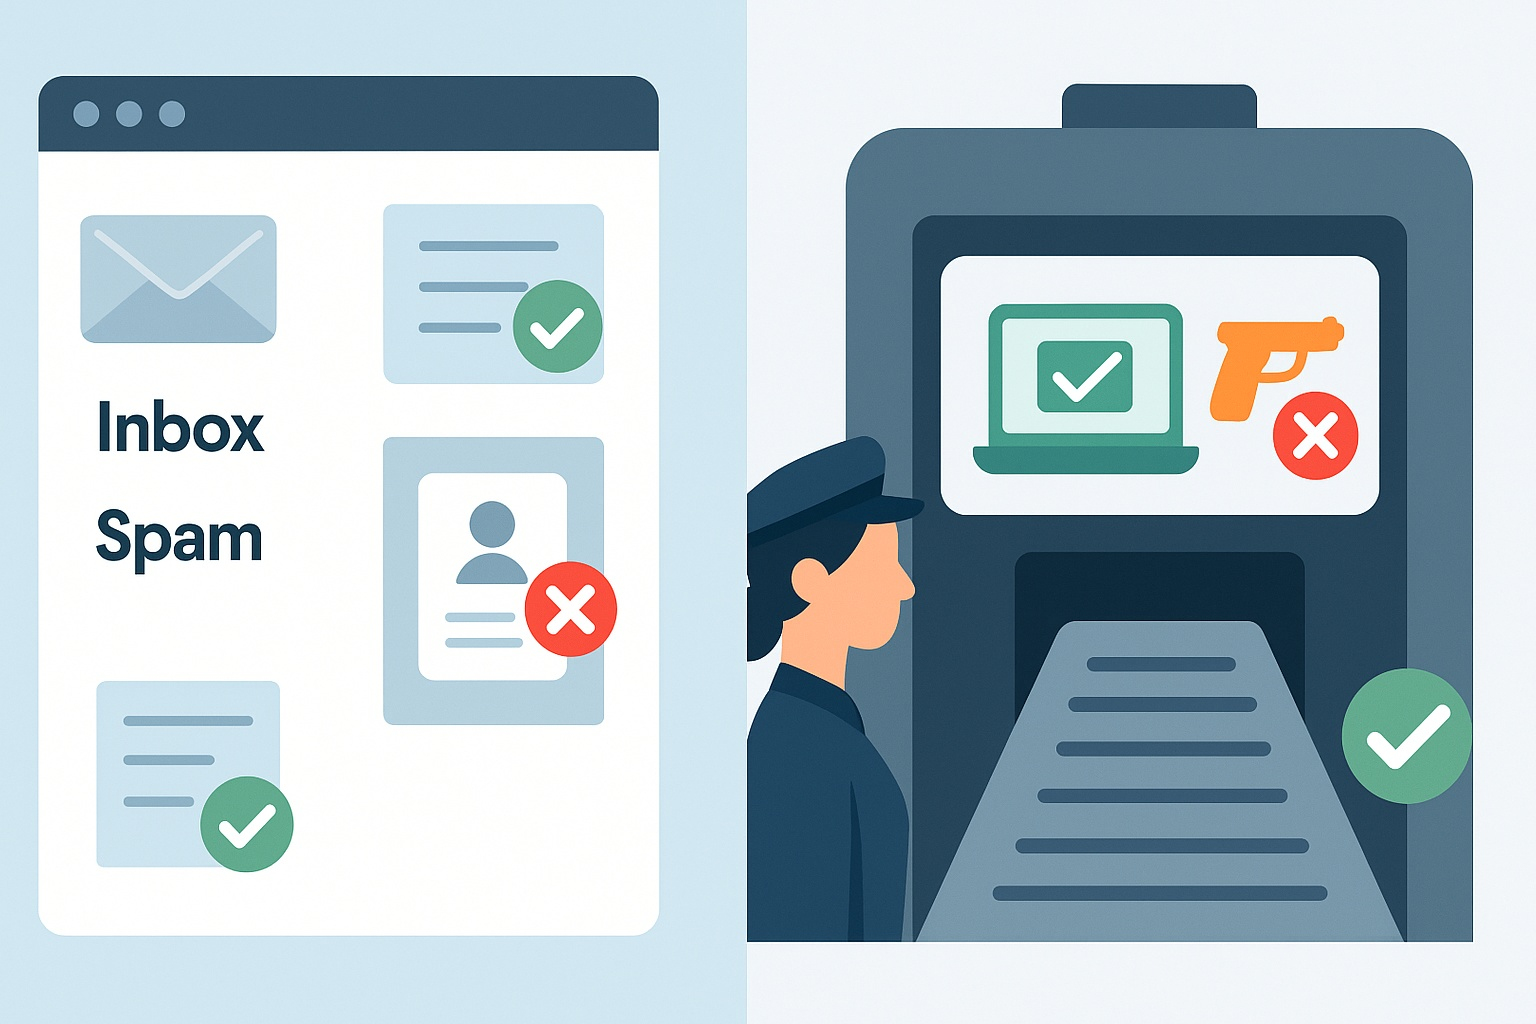
\includegraphics[width=0.5\linewidth]{figure_man/spam_airport.jpg}
    \end{center}
}
  %-----------------------------------------------------------
  \item<2-> \textbf{Multiple objectives:} What if improving one metric worsens another?
    \begin{itemize}
      % \tightlist
      \item \textit{Scalarization}: Combine into one score (e.g.,\ $F_1$)
      \item \textit{Pareto/frontier}: Analyze trade-off without collapsing (e.g., ROC curve)
    \end{itemize}
  %-----------------------------------------------------------
  %\item \textbf{Core performance metrics}
    % \begin{itemize}
    %   \tightlist
    %   \item Precision, Recall, $F_1$
    %   \item Accuracy (misleading on severe class imbalance)
    % \end{itemize}
\end{itemize}

\only<2>{
 \scriptsize
 \renewcommand{\arraystretch}{1.5}
\begin{tabular}{|l|cc|c|}
\hline
\multirow{2}{*}{\textbf{True Values}}
  & \multicolumn{2}{c|}{\textbf{Predicted Values}} & \\%[0.3ex]
  & \textbf{Pos} & \textbf{Neg} & \\[0.3ex]
\hline

\textbf{Pos}
  & \cellcolor[gray]{0.9}\rule{0pt}{3.5ex}TP
  & \cellcolor[gray]{0.9}FN
  & \cellcolor[gray]{0.9}\rule{0pt}{3.5ex}%
    \textbf{Sensitivity/Recall/TPR }%
    $=\dfrac{TP}{TP+FN}$ \\

\textbf{Neg}
  & \cellcolor[gray]{0.9}\rule{0pt}{3.5ex}FP
  & \cellcolor[gray]{0.9}TN
  & \cellcolor[gray]{0.9}\rule{0pt}{3.5ex}%
    \textbf{Specificity }%
    $=\dfrac{TN}{TN+FP}$ \\[0.8ex]
\hline
  & \cellcolor[gray]{0.9}\rule{0pt}{3.5ex}
      \textbf{Precision} $=\dfrac{TP}{TP+FP}$
  & \cellcolor[gray]{0.9}\rule{0pt}{3.5ex}
      \textbf{NPV} $=\dfrac{TN}{TN+FN}$
  % & \cellcolor[gray]{0.9}\rule{0pt}{3ex}%
  %     \textbf{Precision} $=\dfrac{TP}{TP+FP}$
  % & \cellcolor[gray]{0.9}\rule{0pt}{3ex}%
  %     \textbf{NPV} $=\dfrac{TN}{TN+FN}$
  & \cellcolor[gray]{0.9}\rule{0pt}{3.5ex}
      \textbf{F$_1$}%
        $=\dfrac{2\,\text{Precision}\,\text{Recall}}%
                {\text{Precision}+\text{Recall}}$
  %\shortstack[l]{%
      %\tiny\rule{0pt}{3.5ex}\textbf{Accuracy }%
      %  $=\dfrac{TP+TN}{TP+FP+TN+FN}$\\[0.8ex]
      %\tiny\rule{0pt}{3ex}\textbf{F$_1$}%
      %  $=\dfrac{2\,\text{Precision}\,\text{Recall}}%
      %          {\text{Precision}+\text{Recall}}$} 
                \\[0.8ex]
\hline
\end{tabular}
}


%\vspace{0.5em}
% \centering
% 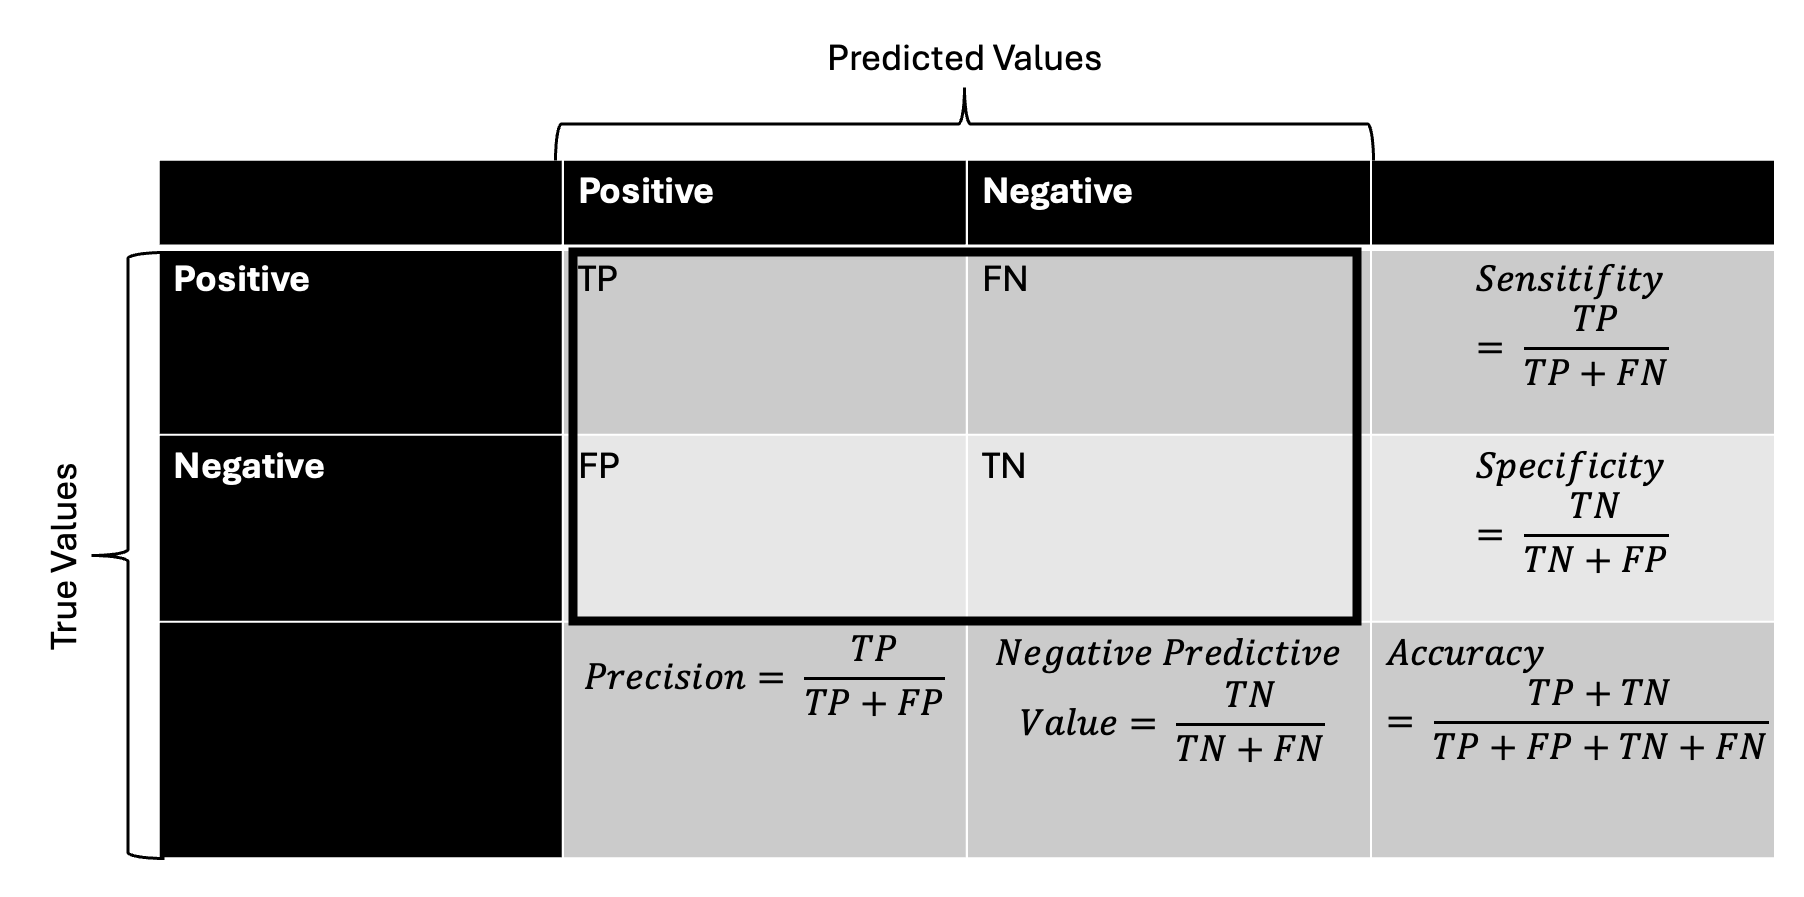
\includegraphics[width=0.65\textwidth]{figure_man/ConfusionMatrix.png}
\end{frame}


% \begin{frame}{Validation Strategy}
% \phantomsection\label{validation-strategy}

% \textbf{Key question}: How to validate the model?

% %from I2ML: https://drive.google.com/file/d/16O-rVIPJVpLIZ9-qb7BRIJxomCXcrNgL/edit
% \begin{figure}[h]
% 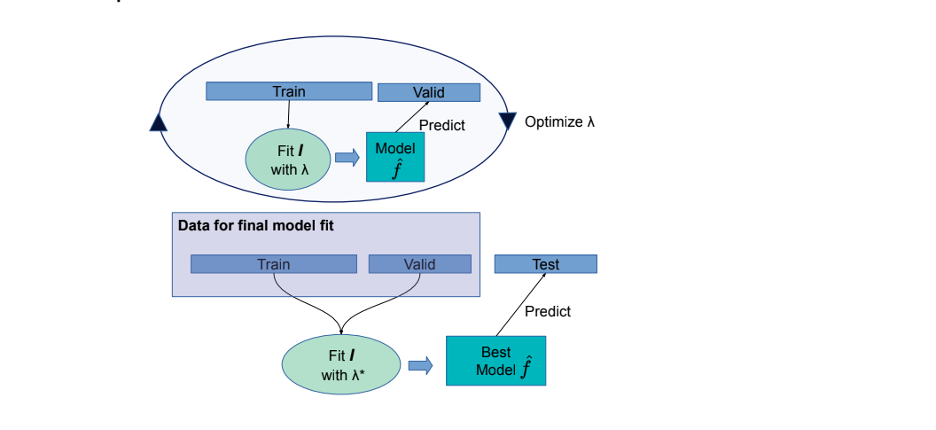
\includegraphics[width=12cm]{figure_man/Validation.png}
% \end{figure}
% \end{frame}

% \begin{frame}{Validation Strategy}
% \phantomsection\label{validation-strategy}

% \textbf{Key question}: How to validate the model?

% Considerations when deciding for a validation strategy:

% \begin{itemize}
% \tightlist
% \item
%   What to generalize to?

%   \begin{itemize}
%   \tightlist
%   \item
%     blocking factors
%   \item
%     temporal effects
%   \item
%     spatial effects
%   \end{itemize}
% \item
%   Validate it just like you would use it in real life:
%   \begin{itemize}
%   \tightlist
%   \item
%     A time series model: You'd build it in 2020 with data from
%     2016--2020, then use it in 2021
%   \item
%     Validate it with the same strategy: Train on 2016--2019, validate on
%     2020
%   \end{itemize}
% \end{itemize}

% \end{frame}

% \begin{frame}{Validation Strategy}
% \phantomsection\label{validation-strategy}

% \textbf{Key question}: How to validate the model?

% be aware of \textbf{data leakage}
% \begin{itemize}
% \tightlist
%     \item Target Leakage: When features that won't be available at prediction time contain information about the target variable.
%     \begin{itemize}
%     \tightlist
%         \item Example: Using "Total Sales in Next Month" as a predictor when trying to forecast sales.
%     \end{itemize} 
%     \item Train-Test Leakage: 
%     \begin{itemize}
%     \tightlist
%         \item Example: Normalizing the dataset using the entire data before splitting into train and test sets.
%     \end{itemize}
% \end{itemize}
% \end{frame}


\begin{frame}{Business Objectives: Validation Strategy}
\phantomsection\label{validation-strategy}

\textbf{Key question}: How to validate the model reliably and realistically?

\textbf{1. Strategic Considerations}
\begin{itemize}
  \item \textbf{What should your model generalize to?}
    \begin{itemize}
      \item \emph{Blocking factors} (e.g., customers, hospitals, product types)
      \item \emph{Temporal effects} (e.g., seasonality, trends)
      \item \emph{Spatial effects} (e.g., regions, branches)
    \end{itemize}

  \item \textbf{Simulate realistic deployment:}
    \begin{itemize}
      \item \textbf{Time series:} Train on data from 2016--2020, deploy in 2021
  \item \textbf{Validation:} Mimic deployment -- train on 2016--2019, validate on 2020
      % \item Time series: Train on 2016--2019, validate on 2020, deploy in 2021
      % \item Match your validation logic to your intended use case
    \end{itemize}
\end{itemize}

\only<1>{
    \begin{center}
        
    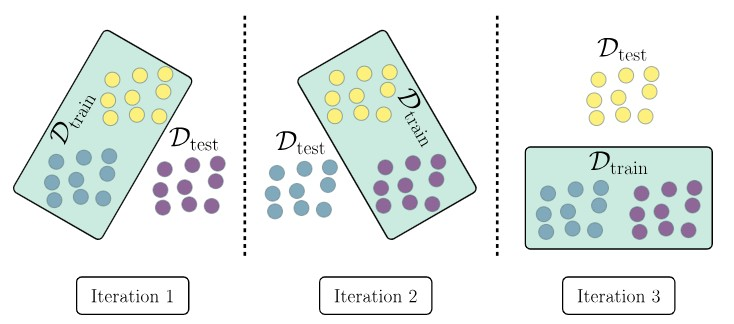
\includegraphics[width=0.5\linewidth]{figure_man/blocking.jpg}
    \end{center}
}
\only<2>{
\textbf{2. Beware of Data Leakage}
\begin{itemize}
  \item \textbf{Target Leakage:} Features leak future info not available at prediction time
    \begin{itemize}
      \item Example: "Total Sales in Next Month" used to predict this month
    \end{itemize}

  \item \textbf{Train-Test Leakage:} Information from the test set is used during training
    \begin{itemize}
      \item Example: Scaling the full dataset before splitting
    \end{itemize}
\end{itemize}
}
%\textbf{Guideline:} Always split your data first, then apply transformations only on training folds.
\end{frame}





% \section{2. Data Acquisition and
% Understanding}\label{data-acquisition-and-understanding-1}

% \begin{frame}{Data Source}
% \phantomsection\label{data-source}
% \textbf{Key question}: Where does the data come from?

% In real world, there are multiple data sources

% \begin{minipage}{0.3\textwidth}
% %https://docs.google.com/presentation/d/1RCourH6lXL6sycgT6HbIXWb7rnQvA5HJ/edit?slide=id.p1#slide=id.p1
% 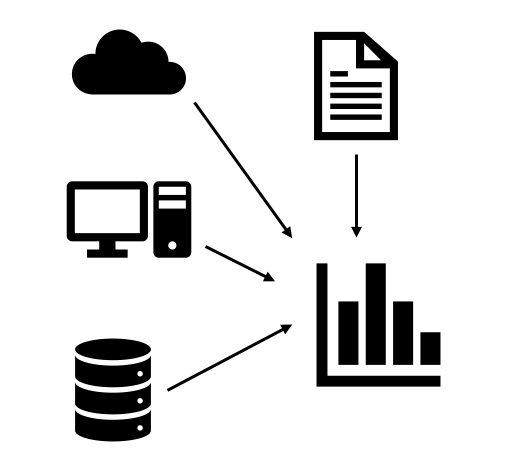
\includegraphics[width=\linewidth]{figure_man/DataSources.png}
% \end{minipage}
% \begin{minipage}{0.6\textwidth}%\RaggedRight
% \begin{itemize}
% %\tightlist
%     \item \textbf{internal vs. external data sources}: external providers might change their data format or discontinue the service
%     \item \textbf{structured vs. unstructured}: structured data can be stored in a database, unstructured one might include images and is not so straightforward to work with
%     \item \textbf{database vs. files}: databases combine many advantages of other file types, most software can grab and process data from there.
%     \item \textbf{on-premise vs. cloud:} decision depends on data protection laws, costs and team preferences
% \end{itemize}
% \end{minipage}

% \end{frame}

\section{2. Data Acquisition and Understanding}\label{data-acquisition-and-understanding}

\begin{frame}{Data Sources and Data Versioning}
\phantomsection\label{data-source}
\textbf{Key question:} What data is available and where does it come from?

\bigskip
\begin{columns}[T]
  \begin{column}{0.35\textwidth}
    \centering
    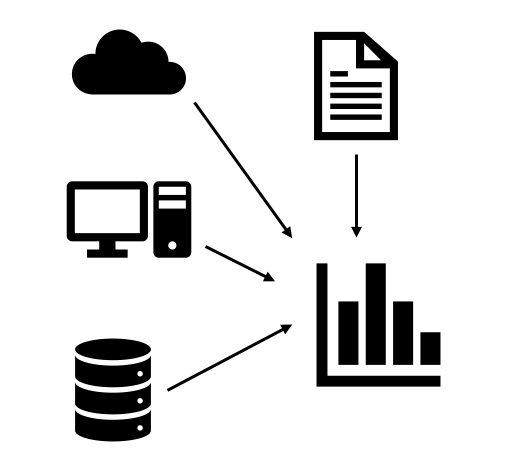
\includegraphics[width=\linewidth]{figure_man/DataSources.png}
  \end{column}

  \begin{column}{0.60\textwidth}
    \begin{itemize}
      % \tightlist
      \item \textbf{Internal vs. External:} External feeds may change format or be discontinued
      \item \textbf{Structured vs. Unstructured:} Tables vs.\ free-text, images, audio, etc.
      \item \textbf{Databases vs. Files:} DBs offer querying, consistency and security
      \item \textbf{On-Premise vs. Cloud:} Governed by regulations, cost and team expertise
    \end{itemize}
  \end{column}
\end{columns}

\textbf{Data Versioning:}

\begin{itemize}
% \tightlist
\item Data can evolve - use version control for data, like \texttt{git} for code  
\item Tools: \texttt{DVC} (Data Version Control), \texttt{Pachyderm}
\end{itemize}



\end{frame}


% \begin{frame}{Data Access at Deployment Time}
% \phantomsection\label{data-access-at-deployment-time}
% \textbf{Key question}: How to feed the \emph{new} data to your model when it's in use?
% \begin{itemize}
% \tightlist
% \item
%   This is often a separate workflow than your training data pipeline
% \item
%   Plan ahead: Think about these questions in the beginning
% \end{itemize}
% \end{frame}



\begin{frame}{Datasheets \furtherreading{GEBRU2018}}
\phantomsection\label{datasheets}

\emph{Datasheets} summarize key metadata about a dataset's content, structure, provenance, and known limitations to support informed and responsible use.

  \begin{itemize}
  % \tightlist
    \item Why and how was the data collected?
    \item What are its limitations and ethical concerns?
    \item For which tasks is it suitable or unsuitable?
  \end{itemize}

\begin{figure}
    \centering
    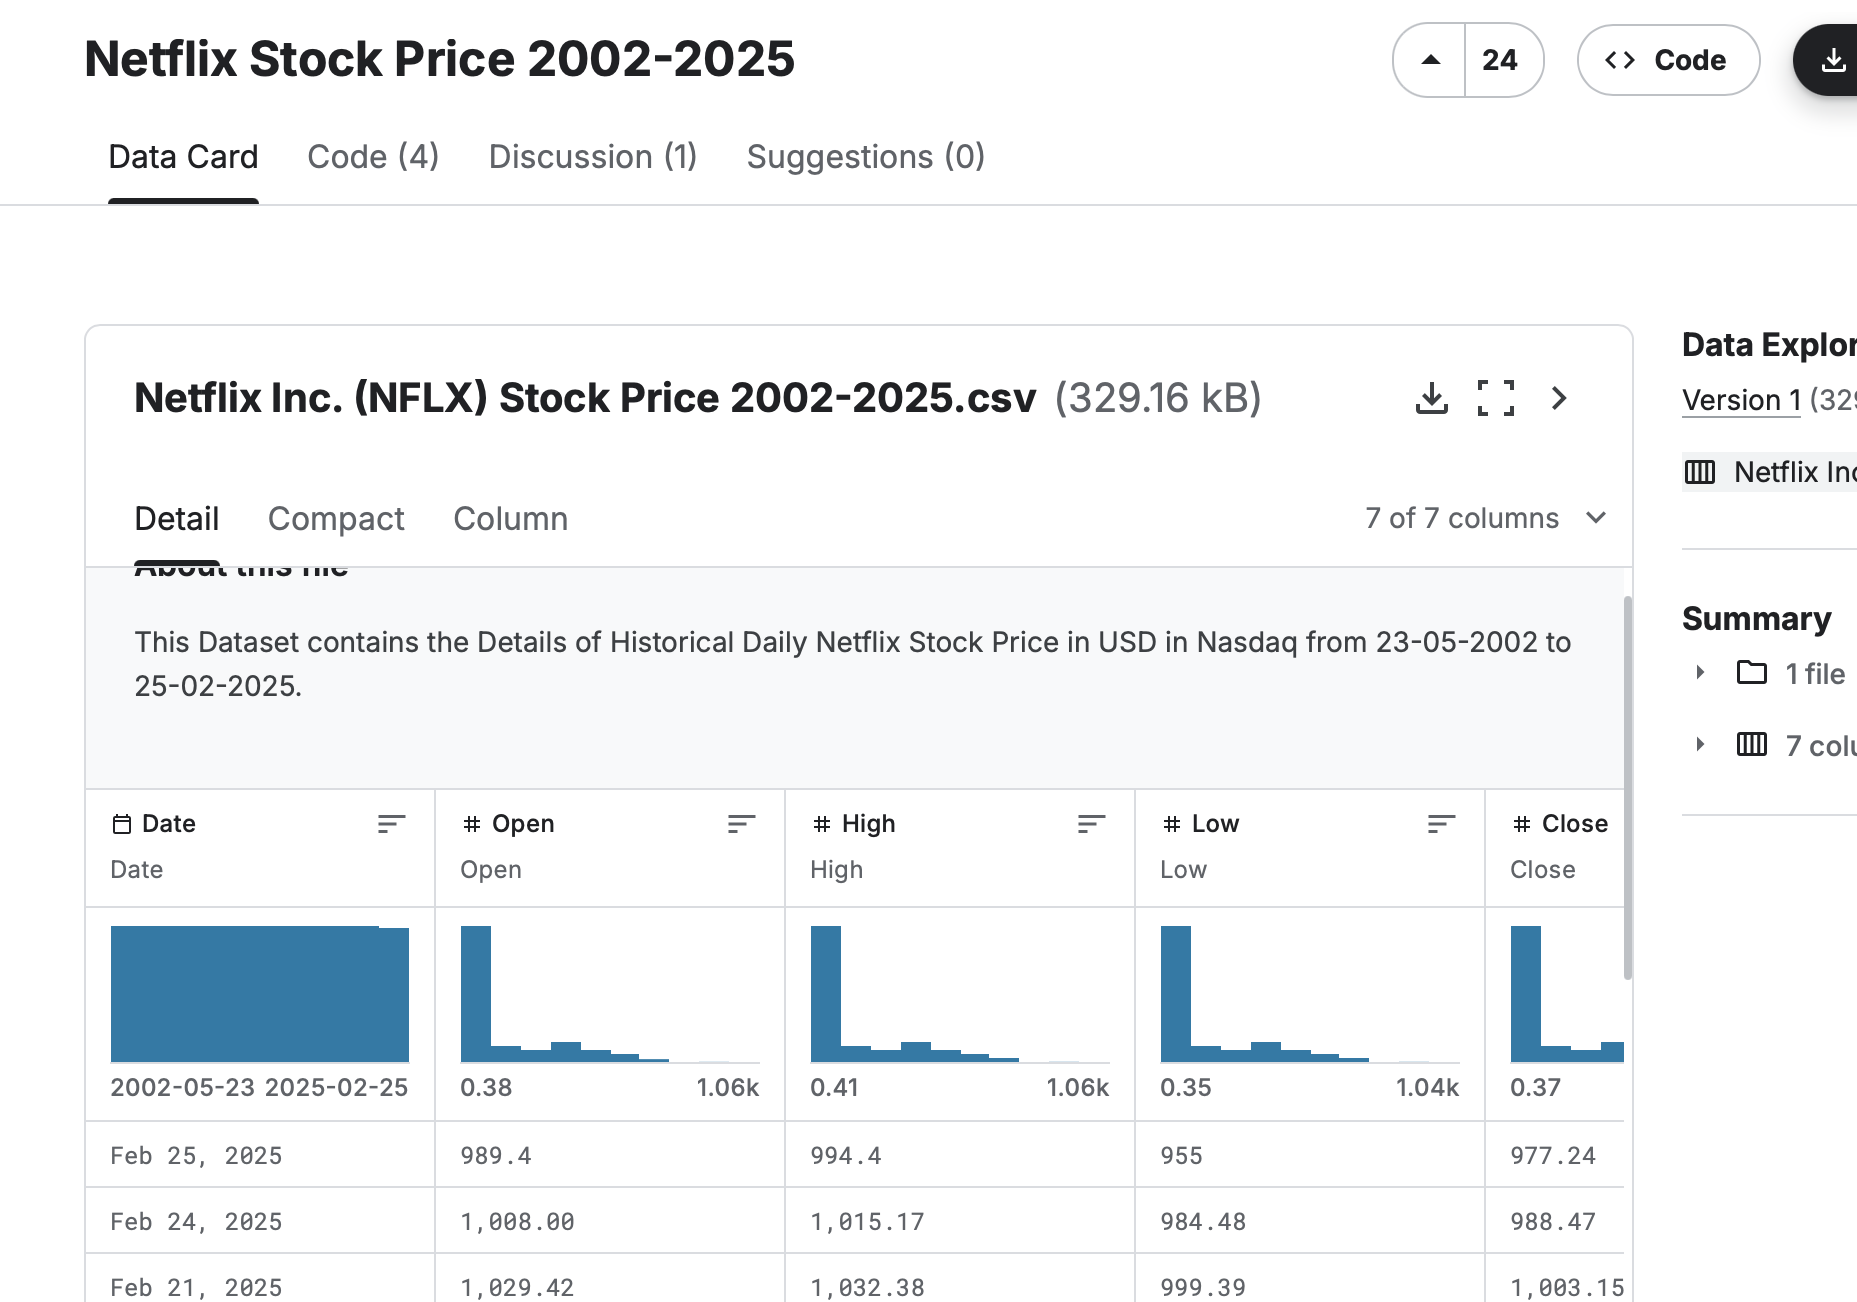
\includegraphics[width=0.6\linewidth]{figure_man/DataSheet.png}\\
\tiny Source: \furtherreading{KAGGLE2025}
\end{figure}

%\scriptsize
%Based on: \href{https://arxiv.org/abs/1803.09010}{Gebru et al., 2018 — Datasheets for Datasets}
\end{frame}

% \begin{frame}{Data Exploration}
% \phantomsection\label{data-exploration}
% \textbf{Key question}: What are the data features and how do they look like?
% \begin{itemize}
% \tightlist
% \item Create a \emph{data dictionary} to clarify:

%   \begin{itemize}
%   \tightlist
% \item Semantic meaning of each feature
%     \item Measurement units and expected ranges
%     \item Valid levels for categorical features (factors)
%     \item Encoding scheme for missing or special values
%   \end{itemize}
% \item  Compute (stratified) summary statistics and inspect missingness
% \item  Plot uni- and bivariate diagrams to explore distributions and structure
% \item Identify: Outliers, anomalies, imbalances, or highly correlated features
% \end{itemize}

% \textbf{Beware of confounders:} Unmeasured variables may bias analysis
% 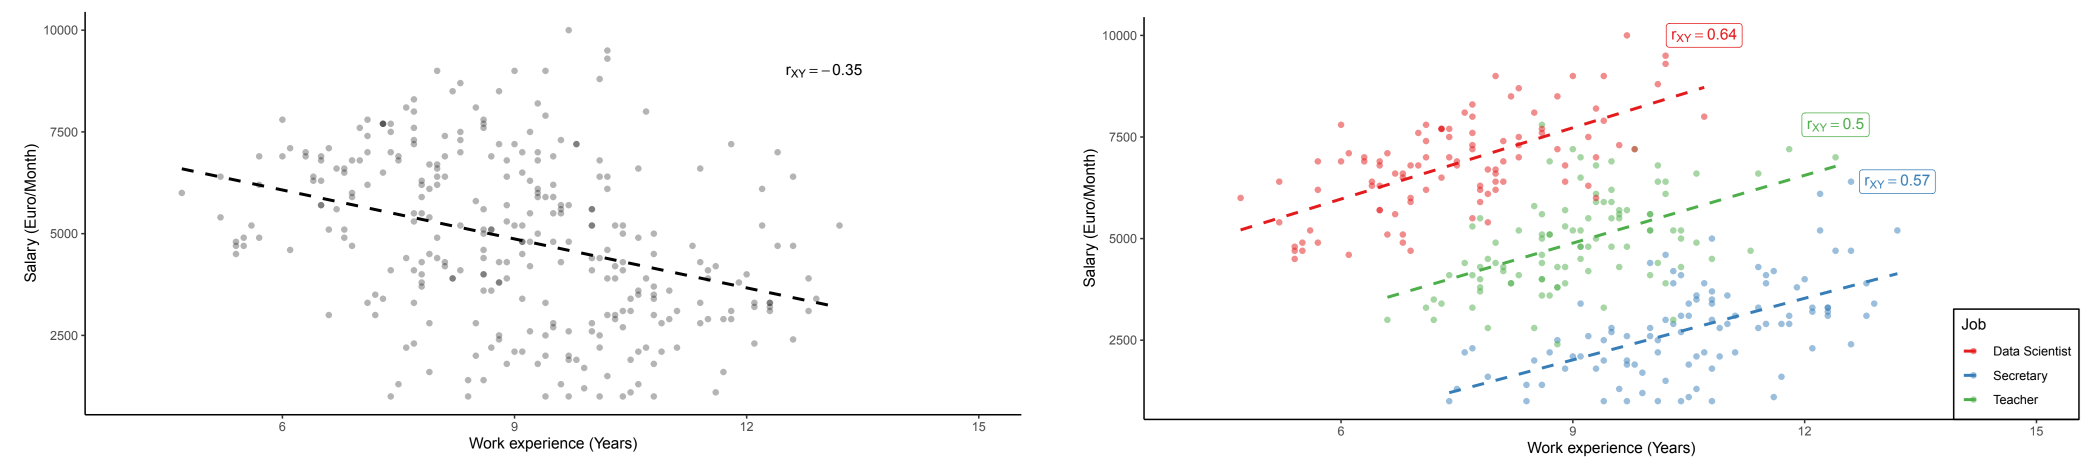
\includegraphics[width = \linewidth]{figure_man/confounder.png}
% \end{frame}

\begin{frame}{Data Exploration}
\phantomsection\label{data-exploration}

\textbf{Key question}: What features are in the data, and what do they reveal?

\begin{itemize}
  \item \textbf{Build a data dictionary}:
  \begin{itemize}
    \item Feature meaning, units, valid ranges/category-levels
    \item Missing value encoding and special codes
  \end{itemize}
  
  \item \textbf{Examine structure and quality to gain understanding}:
  \begin{itemize}
    \item Compute (stratified) summary statistics and inspect missingness
    \item Plot univariate and bivariate distributions
    \item Identify outliers, anomalies, imbalances, redundancy, or high correlation
  \end{itemize}
  
  \item \textbf{Watch for confounders:} unmeasured variables may distort associations
\end{itemize}

\begin{center}
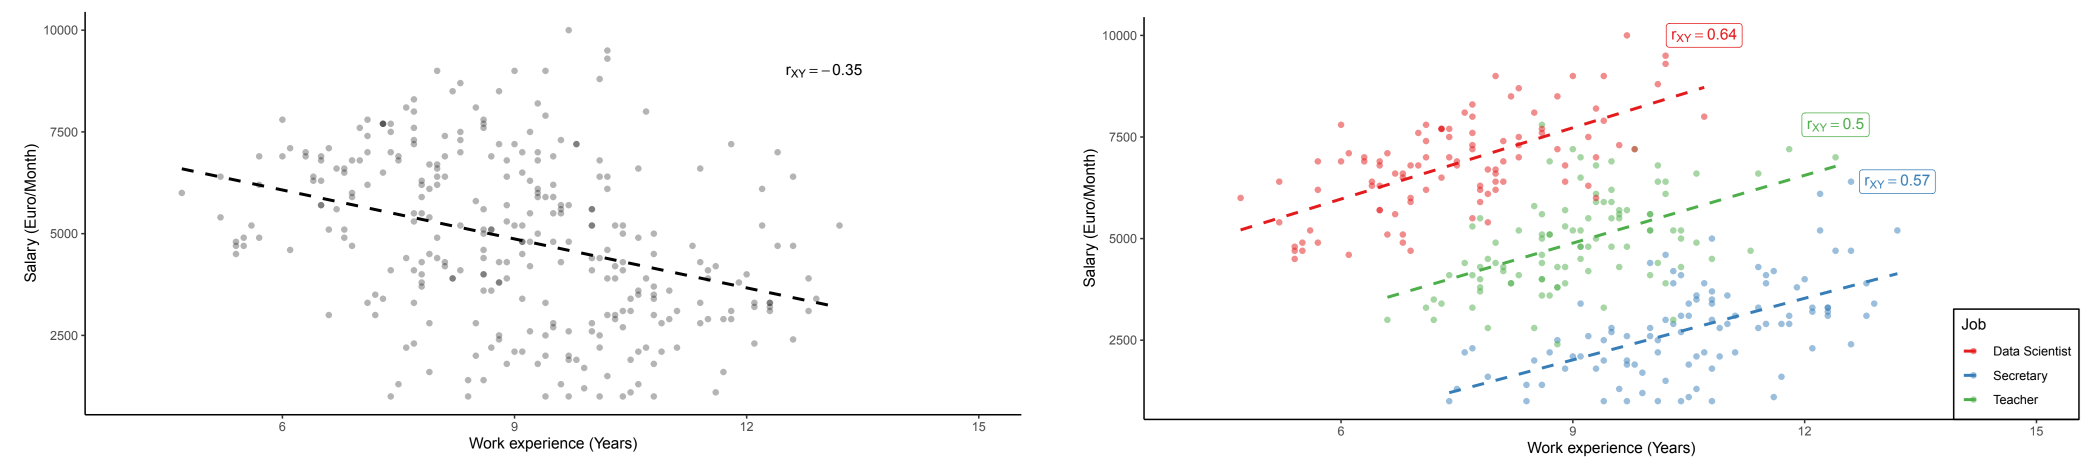
\includegraphics[width=\linewidth]{figure_man/confounder.png}
\end{center}
\end{frame}

\begin{frame}{Data Quality}
\phantomsection\label{data-quality}
\textbf{Key question:} Is the data fit for modeling? \emph{Garbage in, garbage out.}

\begin{itemize}
  \item Assess missingness: How many values are missing, and where?
  \item Detect implausible or inconsistent values (requires domain expertise)
  \item Standardize formats (e.g., date/time parsing)
  \item Drop near-constant or non-informative features
  \item Remove redundancy and obsolete variables
\end{itemize}

\vspace{0.5em}
\textbf{Watch for data bias:}
\begin{itemize}
  \item \textit{Sampling bias:} E.g., a survey at 10am in the city center misses working adults
  \item \textit{Response bias:} Online reviews often reflect extreme opinions, not the median
\end{itemize}
\end{frame}






% \begin{frame}[fragile]{Hidden Features}
% \phantomsection\label{hidden-features}
% \begin{itemize}
% \tightlist
% \item
%   Also known as \emph{confounder variables} (or \emph{mediator
%   variables} in psychology)
% \item
%   Variables that influence your target outcome, but that you
%   didn't measure
% \item
%   Simple example:

%   \begin{itemize}
%   \tightlist
%   \item
%     A customer happiness survey done over 7 days concludes that
%     customers are very unhappy on Fridays and Saturdays
%   \item
%     Hidden feature: There was a rainstorm on these two days
%   \item
%     The hidden feature \texttt{weather}, not the weekday, was
%     responsible for the drop in happiness
%   \end{itemize}
% \item
%   As a more realistic example, data measured over multiple facilities
%   may contain a similar bias, when measurement devices have slight
%   differences in those locations
% \end{itemize}
% \end{frame}

% \begin{frame}{Pipeline}
% \phantomsection\label{pipeline}
% 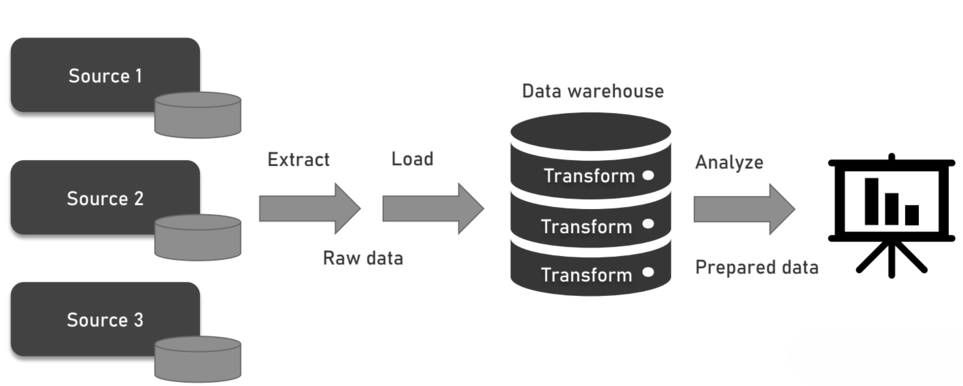
\includegraphics[width = 0.5\linewidth]{figure_man/pipeline.png}
% \begin{itemize}
% \tightlist
% \item
%   You usually need to set up a pipeline to ingest new data and refresh
%   your existing data set regularly.
% \item
%   A pipeline can be

%   \begin{itemize}
%   \tightlist
%   \item
%     batch-based
%   \item
%     streaming or real-time
%   \item
%     a hybrid of these two
%   \end{itemize}
% \end{itemize}
% \textbf{Data Versioning} can make sense, as data changes over time
% \begin{itemize}
% \tightlist
% \item
%   Like version control for code (e.g. Git), it can make sense to have version control for your data sets
% \item
%   \emph{Pachyderm} and \emph{DVC} (Data Version Control) are two
%   versioning tools
% \end{itemize}
% \end{frame}


% \begin{frame}{Hidden Complexity in Data}
% \phantomsection\label{hidden-complexity}

% \vspace{0.5em}
% \begin{itemize}
%   \item \textbf{Hidden Features:} Unmeasured variables (e.g., confounders) may bias analysis
%   \end{itemize}
% 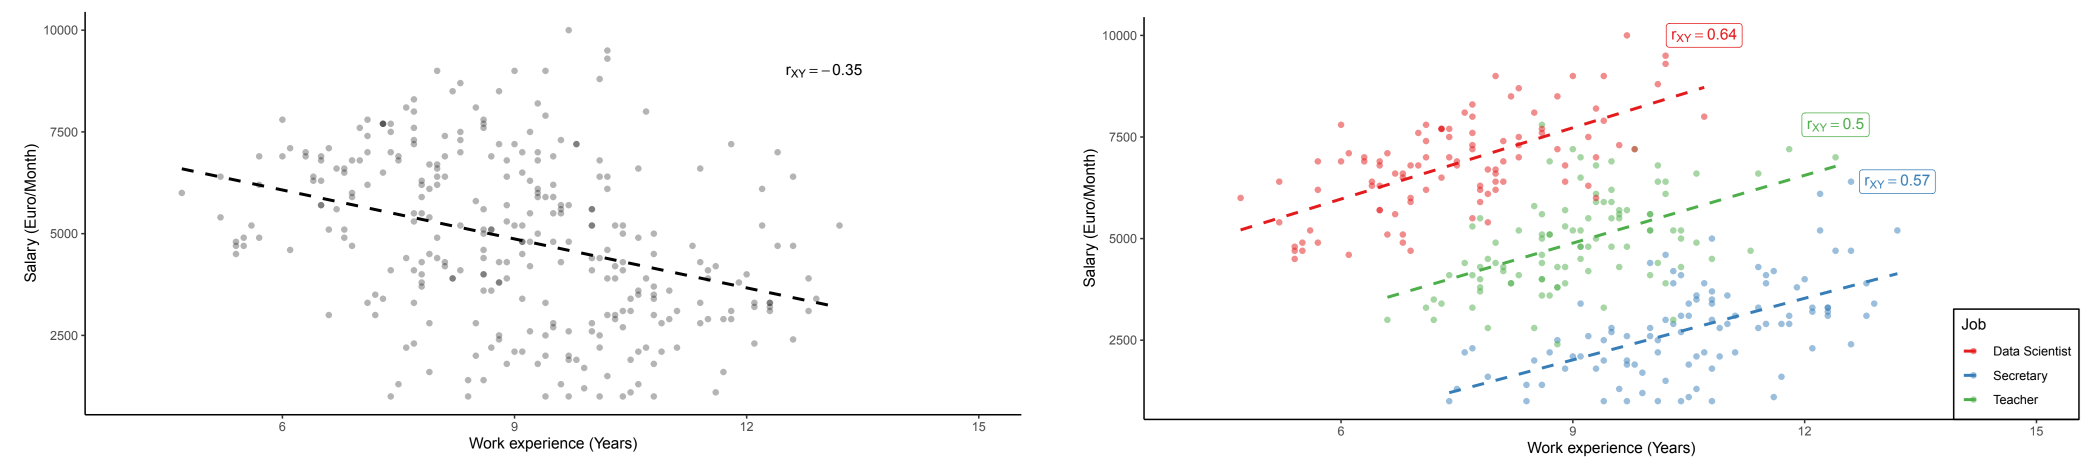
\includegraphics[width = \linewidth]{figure_man/confounder.png}
%   % \begin{itemize}
%   %   \item Example: Low customer satisfaction on Friday/Saturday may be due to \texttt{weather}, not weekday
%   %   \item Real-world case: Subtle biases across facilities due to sensor differences
%   % \end{itemize}
%   \vspace{-1em}
%   \pause
% \begin{itemize}
%   \item \textbf{Data Pipelines:} Ensure consistent and reproducible data ingestion
%   \begin{columns}[T, totalwidth=\textwidth]
%       \begin{column}{0.38\textwidth}
%           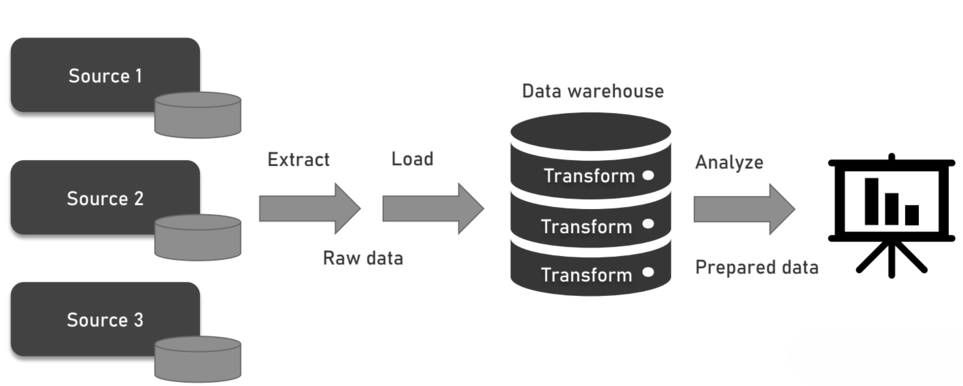
\includegraphics[width = \linewidth]{figure_man/pipeline.png}
%       \end{column}
%             \begin{column}{0.62\textwidth}
%             \begin{itemize}
%     \item Can be batch-based, streaming, or hybrid
%     \item Should support automated refresh \& monitoring
%     \item \textbf{Data Versioning} helps track changes over time (e.g., with \texttt{DVC}, \texttt{Pachyderm})
%   \end{itemize}
%       \end{column}
%   \end{columns}

% \end{itemize}

% \vspace{0.5em}
% \textit{Key message: Understanding your data requires both domain awareness and engineering discipline.}
% \end{frame}



% \begin{frame}{Data Governance and Security}
% \phantomsection\label{data-governance-and-security}
% \textbf{Key question}: How to keep the data secure, accurate and usable?
% \begin{itemize}
% \tightlist
%     \item \textbf{Integrity}: encure data stays intact when being updated (no duplicates,...)
%     \item \textbf{Access}: ensure pipeline allows constant access
%     \item establish internal rules for data use
%     \item make sure to meet legal requirements such as privacy, anonymization
% \end{itemize}
% \end{frame}

% \begin{frame}{Wrangling, Exploration and Cleaning}
% \phantomsection\label{wrangling-exploration-and-cleaning}
% \begin{itemize}
% \tightlist
% \item
%   Once you successfully ingested the necessary data, you can begin to
%   prepare it for modeling
% \item
%   This preparation often takes up most of the time in a ML project
% \item
%   The necessary steps include exploratory data analysis (EDA), data
%   wrangling (e.g.~joins) and data cleaning
%   \item Sometimes the data you obtain is not yet labeled $\rightarrow$ you need humans (with domain knowledge) to assign labels to your data points
  
% \end{itemize}
% \end{frame}


\section{3. Modeling}\label{modeling-1}

% \begin{frame}{Modeling Steps Overview}
% %https://docs.google.com/presentation/d/1RCourH6lXL6sycgT6HbIXWb7rnQvA5HJ/edit?slide=id.p1#slide=id.p1
% 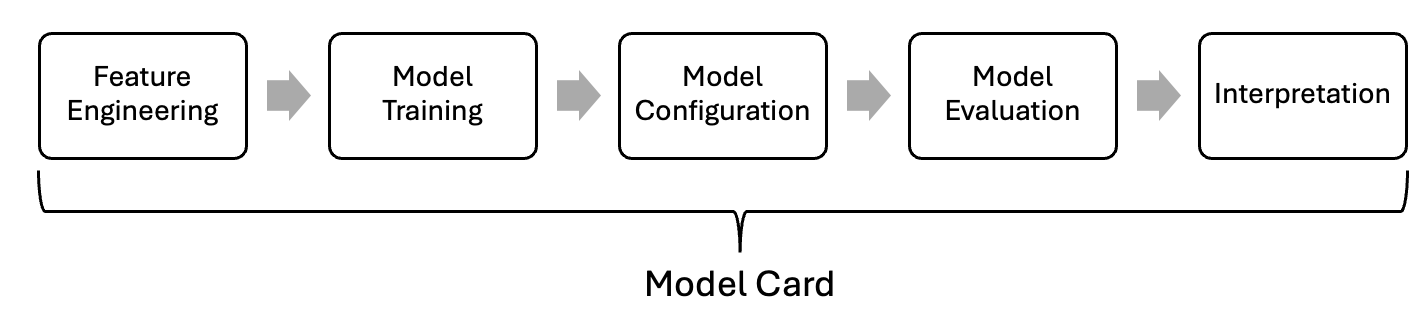
\includegraphics[width=\linewidth, trim=0 60 0 0, clip]{figure_man/Modelling1.png}
    
% \end{frame}

\begin{frame}[t]{Feature Engineering}
\phantomsection\label{feature-engineering}
%https://docs.google.com/presentation/d/1RCourH6lXL6sycgT6HbIXWb7rnQvA5HJ/edit?slide=id.p1#slide=id.p1
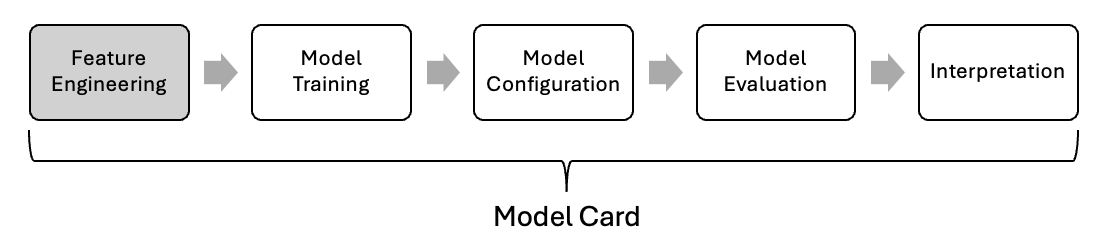
\includegraphics[width = \linewidth, trim=0 60 0 0, clip]{figure_man/Modelling2.png}

\textbf{Feature Engineering} transforms raw data into informative input variables for modeling.

\begin{itemize}
% \tightlist
  \item \textbf{Transformation}: Scaling, log-transform, one-hot encoding
  \item \textbf{Selection}: Wrapper and filter methods, model-based importance
  \item \textbf{Dimensionality Reduction}: PCA, t-SNE
  \item \textbf{Creation}: Aggregation, binning, interaction terms
\end{itemize}

\textbf{Best Practices:}
\begin{itemize}
% \tightlist
  \item Avoid overengineering: irrelevant features introduce noise
  \item Fit transformations \textbf{only on training data}; reuse parameters for test data
  \item Prevent leakage: never use test data in feature construction
\end{itemize}

\end{frame}

\begin{frame}[t]{Model Training}
\phantomsection\label{model-training}

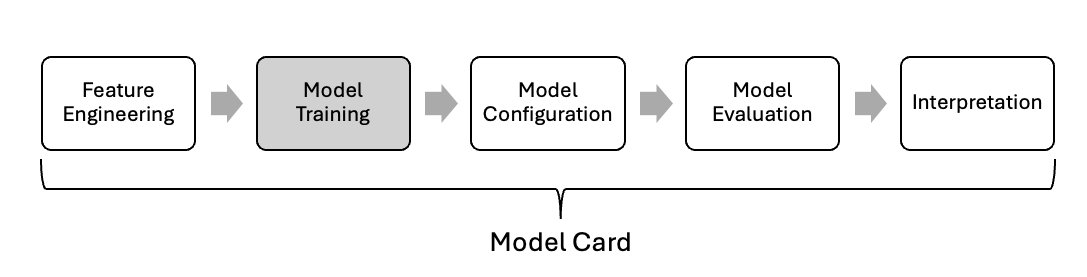
\includegraphics[width=\linewidth, trim=0 60 0 0, clip]{figure_man/Modelling3.png}

\vspace{0.5em}
Treat model training like a scientific experiment:
\begin{itemize}
% \tightlist
  \item \textbf{Track all inputs precisely:}
    \begin{itemize}
    % \tightlist
      \item Dataset version
      \item Algorithm and hyperparameters
      \item Code version (e.g., Git commit/tag)
    \end{itemize}
  \item \textbf{Proceed iteratively:}
    \begin{itemize}
    % \tightlist
      \item \emph{Start simple} – build a fast, interpretable baseline
      \item Gradually increase model complexity and validate each improvement
    \end{itemize}
\end{itemize}
\end{frame}

% \begin{frame}[t]{Model Configuration}
% \phantomsection\label{model-configuration}
% %https://docs.google.com/presentation/d/1RCourH6lXL6sycgT6HbIXWb7rnQvA5HJ/edit?slide=id.p1#slide=id.p1
% 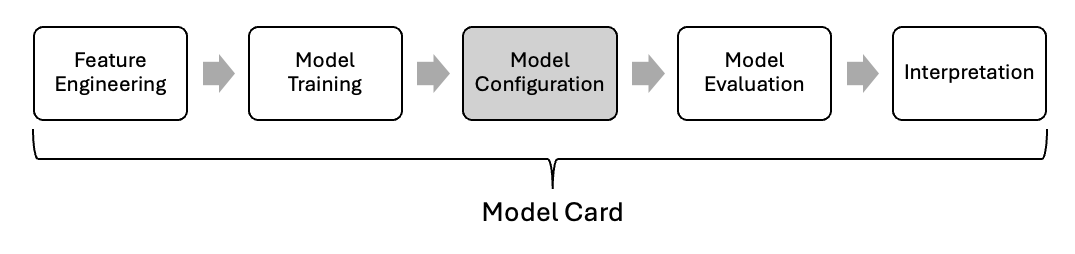
\includegraphics[width = \linewidth, trim=0 60 0 0, clip]{figure_man/Modelling4.png}
% \begin{itemize}
% \tightlist
% \item
%   How do you store a configuration setup you used for a specific
%   experiment (model)?\\
%   \(\rightarrow\) And how do you store \emph{small} changes to that
%   setup?
% \item
%   This configuration should be stored and clearly readable (i.e.~in
%   plain text or json)
% \item
%   Good tools can help, e.g.~\href{https://hydra.cc}{hydra}
% \end{itemize}
% \end{frame}

\begin{frame}[t]{Model Configuration}
\phantomsection\label{model-configuration}

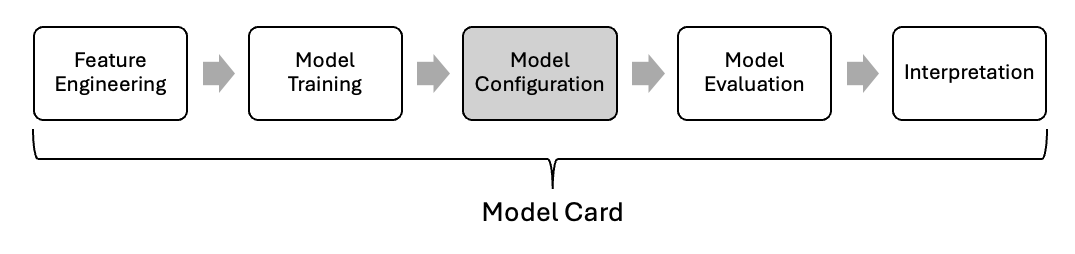
\includegraphics[width=\linewidth, trim=0 60 0 0, clip]{figure_man/Modelling4.png}

\vspace{0.5em}
\begin{itemize}
% \tightlist
  \item How do you track the exact configuration of a model experiment?
  \item How do you record small changes between experiments?
  \item Store in plain text (e.g., \texttt{.yaml}, \texttt{.json}) for readability and version control
\item Recommended tool: structured configuration managers
    \begin{itemize}
    % \tightlist
      \item \textbf{Python}: \furtherreading{HYDRA} - structured, hierarchical configuration management
      \item \textbf{R}: \furtherreading{RCONFIG} - environment-based YAML setup
    \end{itemize}
\end{itemize}
\end{frame}


% \begin{frame}[t]{Model Evaluation}
% \phantomsection\label{model-evaluation}
% %https://docs.google.com/presentation/d/1RCourH6lXL6sycgT6HbIXWb7rnQvA5HJ/edit?slide=id.p1#slide=id.p1
% 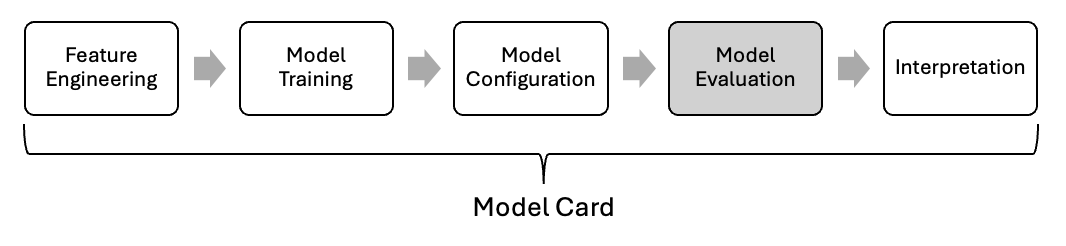
\includegraphics[width = \linewidth, trim=0 60 0 0, clip]{figure_man/Modelling5.png}
% \begin{itemize}
% \tightlist
% \item
%   To select the best model, evaluate based on the
%   \textbf{metrics} you predefined
% \item Use the test or validation data set according to the validation method predefined
% \item
%   Besides this performance scoring, you can evaluate your
%   model's \textbf{robustness}: How sensitive is it to noise or other pertubations
%   and adverserial attacks?

%   \begin{itemize}
%   \tightlist
%   \item
%     Add random noise to your dataset and investigate the impact
%     on your model's parameters and/or performance
%   \end{itemize}
% \end{itemize}
% \end{frame}

\begin{frame}[t]{Model Evaluation}
\phantomsection\label{model-evaluation}

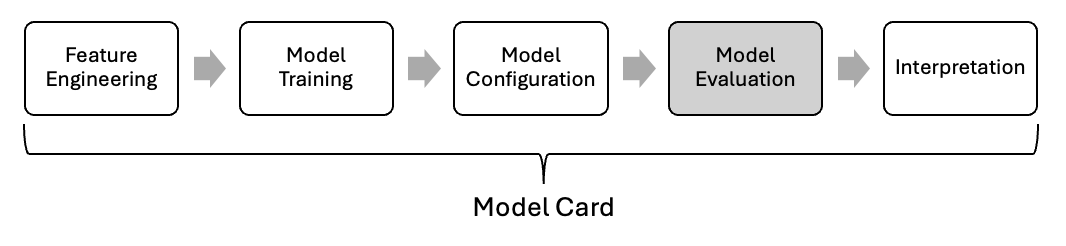
\includegraphics[width=\linewidth, trim=0 60 0 0, clip]{figure_man/Modelling5.png}

\vspace{0.5em}
\begin{itemize}
% \tightlist
  \item Select models based on predefined \textbf{metrics} (e.g., accuracy, AUC, RMSE)
  \item Use the \textbf{validation or test set} in line with your validation strategy
  \item Assess \textbf{robustness}: How does the model respond to noise, perturbations, or adversarial inputs?\\
  $\Rightarrow$ Add synthetic noise and measure changes in model parameters/performance
\end{itemize}
\end{frame}


% \begin{frame}[t]{Interpretation}
% \phantomsection\label{interpretation}
% %https://docs.google.com/presentation/d/1RCourH6lXL6sycgT6HbIXWb7rnQvA5HJ/edit?slide=id.p1#slide=id.p1
% 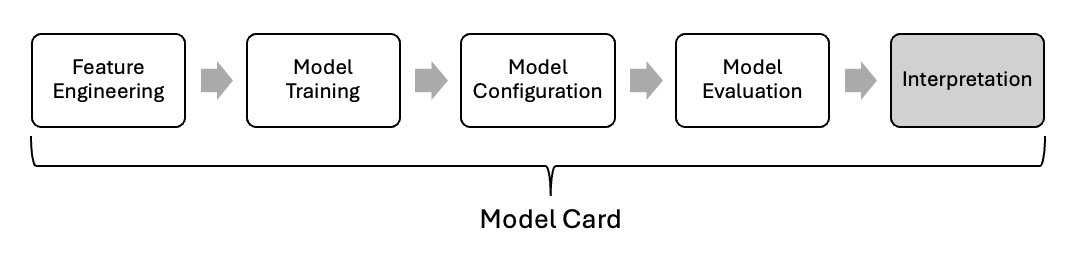
\includegraphics[width = \linewidth, trim=0 60 0 0, clip]{figure_man/Modelling6.png}
% To understand your model better, you can use methods from
%   \textbf{Interpretable Machine Learning (IML)}
% \begin{itemize}
% \tightlist
%     \item Feature importances: how much did each feature contribute to the prediction?
%     \item uncover potential algorithmic biases:
%     \begin{itemize}
%     \tightlist
%         \item E.g., in October 2018
%     \href{https://www.theguardian.com/technology/2018/oct/10/amazon-hiring-ai-gender-bias-recruiting-engine}{world
%     headlines reported} about an Amazon AI recruiting tool that favored
%     men. Amazon's model was trained on biased data that were skewed
%     towards male candidates. It has built rules that penalized resumes
%     that included the word ``women's''.
%     \end{itemize}
% \end{itemize}
% \end{frame}

\begin{frame}[t]{Interpretation and Fairness}
\phantomsection\label{interpretation}

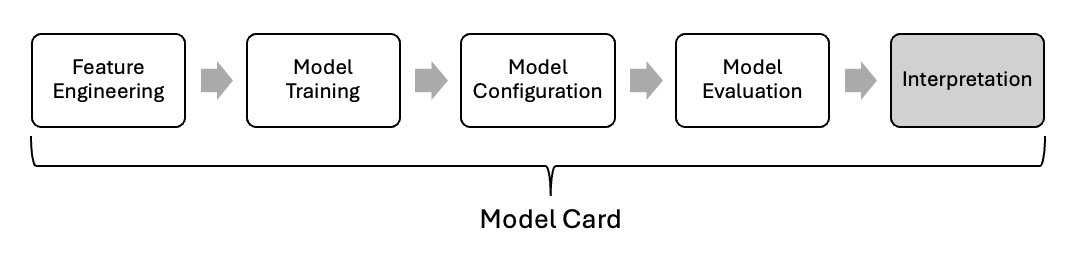
\includegraphics[width=\linewidth, trim=0 60 0 0, clip]{figure_man/Modelling6.png}

\vspace{0.5em}
To understand and trust your model, apply methods from \textbf{Interpretable Machine Learning (IML)}:
\begin{itemize}
% \tightlist
  \item \textbf{Feature Importance}: Which features drive predictions globally?
  \item \textbf{Effects \& Interactions}: Visualize marginal effects and feature interactions %(e.g., ALE, PDP)
  \item \textbf{Local Explanations}: Explain individual predictions %(e.g., LIME, SHAP)
  \item \textbf{Bias Detection}: Reveal fairness issues and unintended discrimination
    \begin{itemize}
    % \tightlist
      \item Example: Amazon's 2018 hiring tool penalized resumes with “women's” due to biased training data % OLD
%\citebutton{The Guardian, 2018}{https://www.theguardian.com/technology/2018/oct/10/amazon-hiring-ai-gender-bias-recruiting-engine}
% NEW
\furtherreading{GUARDIAN2018}
    \end{itemize}
\end{itemize}
\end{frame}


\begin{frame}{Model Cards  for
  Model Reporting % OLD
%\citebutton{Mitchell et al. 2019}{https://arxiv.org/pdf/1810.03993.pdf}
% NEW
\furtherreading{MITCHELL2019}}
\phantomsection\label{model-cards}
%https://docs.google.com/presentation/d/1RCourH6lXL6sycgT6HbIXWb7rnQvA5HJ/edit?slide=id.p1#slide=id.p1
%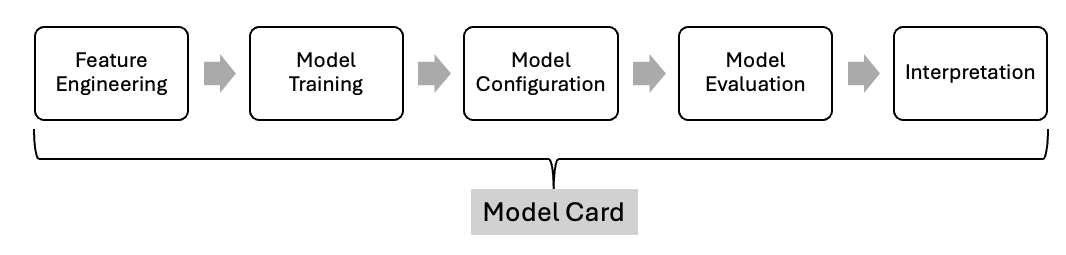
\includegraphics[width = \linewidth, trim=0 60 0 0, clip]{figure_man/Modelling7.png}
\textbf{Model Card}: Documentation of the model similar to a Datasheet for data

\begin{columns}[T, totalwidth=\textwidth]
  \begin{column}{0.4\textwidth}
    \begin{itemize}
    %\tightlist
      \item \textbf{Model Details}: Algorithm, parameters, model version
      \item \textbf{Intended Use}: Intended use and out-of-scope use cases
      \item \textbf{Performance}: Key metrics, validation approaches
      \item \textbf{Analyses}: Feature/target distributions in train/test data
      \item \textbf{Ethical Considerations}: Failure modes, fairness concerns, inappropriate use
    \end{itemize}
  \end{column}
  \begin{column}{0.6\textwidth}
    \centering
    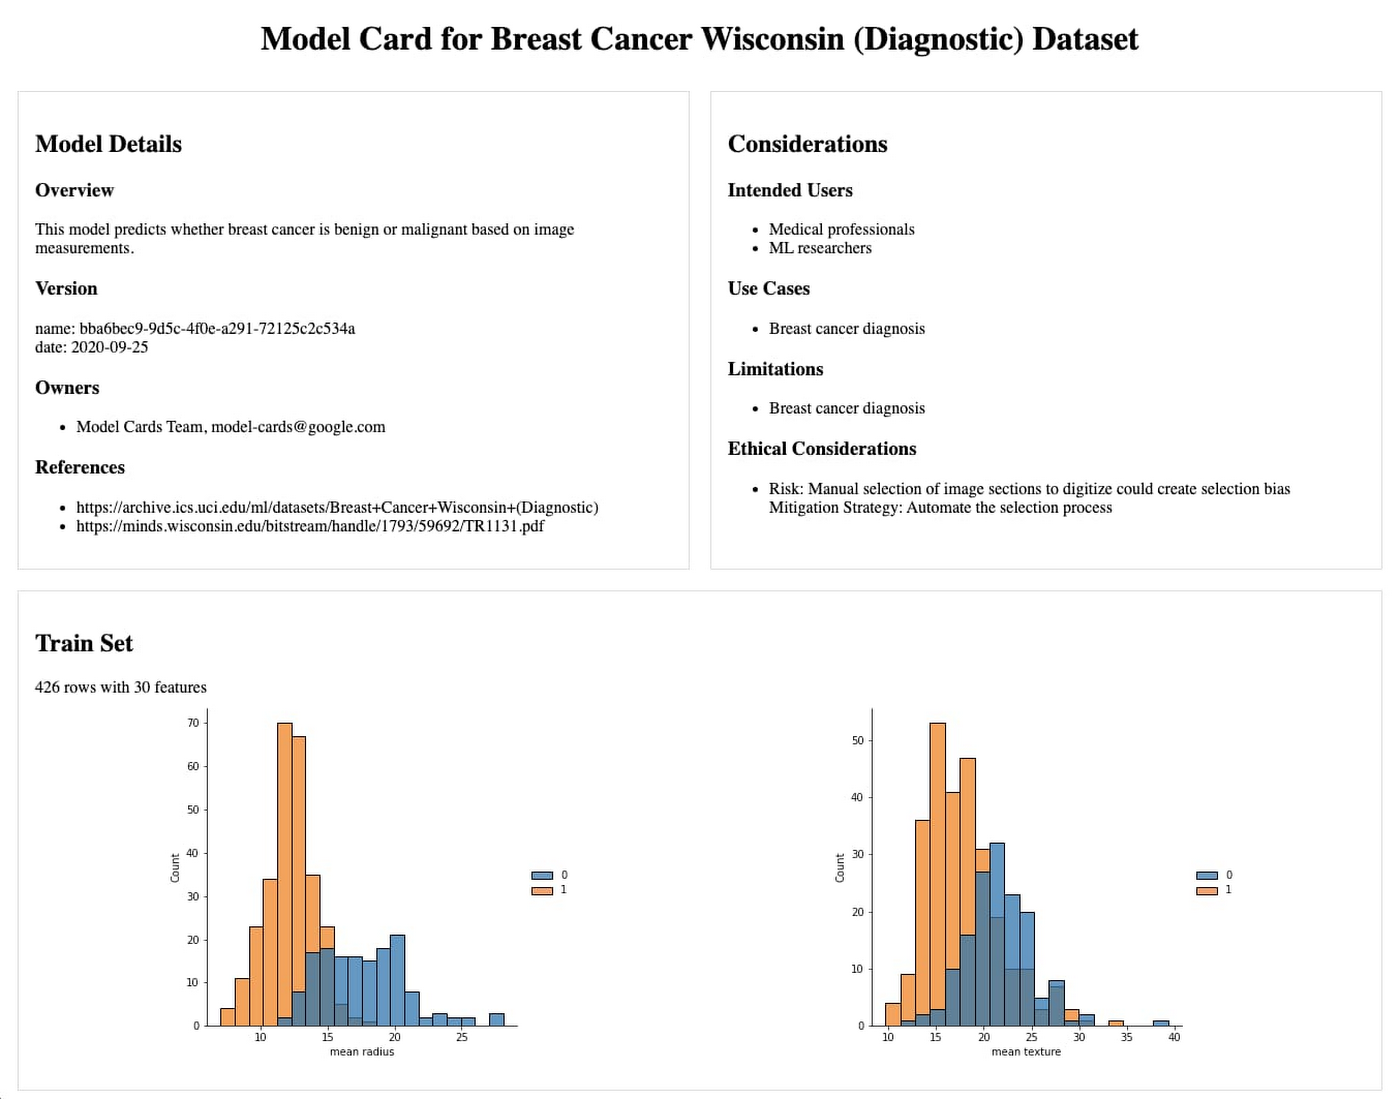
\includegraphics[width=\linewidth]{figure_man/modelcard.png}
  \end{column}
\end{columns}

\end{frame}

\section{4. Model Governance}\label{model-governance-1}

% \begin{frame}{Model Governance}
% \phantomsection\label{model-governance-2}
% \begin{quote}
% Developing and deploying ML systems is relatively fast and cheap, but
% maintaining them over time is difficult and expensive.
% ~\href{https://papers.nips.cc/paper/5656-hidden-technical-debt-in-machine-learning-systems.pdf}{Hidden
% Technical Debt in ML Systems}
% \end{quote}
% \end{frame}

% \begin{frame}{Model Governance}
% \phantomsection\label{model-governance-3}
% \begin{itemize}
% \tightlist
% \item
%   Model Governance includes the \textbf{people, processes and
%   technologies} needed to manage and protect your ML model.
% \item it ensures easy maintenance and possibilities for adaption
% \item
%   Two extremes have to be avoided:

%   \begin{itemize}
%   \tightlist
%   \item
%     \textbf{Repression} by too many standards, rules, and controlling
%   \item
%     \textbf{Chaos} by too much speed, freedom, creativity and change
%   \end{itemize}
% \end{itemize}
% \end{frame}

\begin{frame}{Model Governance}
\phantomsection\label{model-governance-3}


\begin{itemize}
% \tightlist
  \item Model Governance includes \textbf{people, processes, and technologies} needed to manage and protect your ML models.
    \item Ensures long-term maintainability and adaptation as requirements evolve.
  \item Two extremes must be avoided:
    \begin{itemize}
    % \tightlist
      \item \textbf{Repression}: too many rules, rigid standards, excessive control
      \item \textbf{Chaos}: too much speed, freedom, creativity, and unstructured change
    \end{itemize}
  %\item Good governance ensures your models remain \textbf{maintainable}, \textbf{adaptable}, and usable over time - even as requirements evolve.
\end{itemize}

    Model governance steps are:
    %https://docs.google.com/presentation/d/1RCourH6lXL6sycgT6HbIXWb7rnQvA5HJ/edit?slide=id.p1#slide=id.p1
    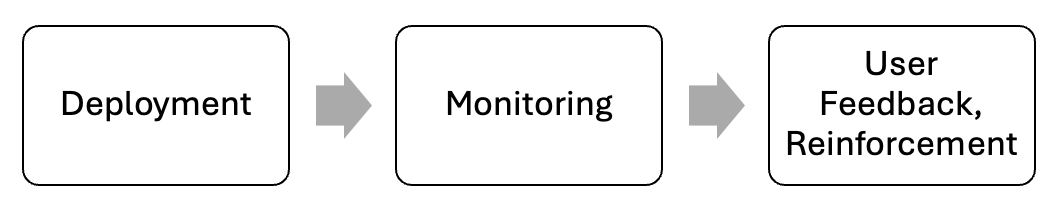
\includegraphics[width = \linewidth]{figure_man/Model Governace.png}

    
\begin{quote}
\footnotesize
"Developing and deploying ML systems is relatively fast and cheap, but
maintaining them over time is difficult and expensive."
\hfill~\furtherreading{HIDDENDEBT}
\end{quote}
\end{frame}

% \begin{frame}{Deployment}
% \phantomsection\label{deployment}
% %TODO include graphics on deployment strategies
% \textbf{Deployment}: make model accessible to users (humans or other programs)
% \begin{itemize}
% \tightlist
% \item
%   You can deploy your model in different ways:

%   \begin{itemize}
%   \tightlist
%   \item
%     \textbf{One-off}: If you only need your model trained once (or very
%     rarely), train it by hand and push it to production
%   \item
%     \textbf{Batch}: With batch training, you constantly (e.g.~weekly)
%     update your model with a new batch of data (e.g.~this week's new
%     contracts)
%   \item
%     \textbf{Real-time}: Some models are very time-critical and need to
%     be updated continously on a stream of data.
%   \end{itemize}
% \item If you retrain and update your model frequently, it makes sense to have some model \textbf{versioning}
% \begin{itemize}
% \tightlist
%     \item \href{https://mlflow.org/}{MLflow} is an open source platform for ML
%   lifecycle management that includes a model registry
% \end{itemize}
% \end{itemize}
% \end{frame}

\begin{frame}{Deployment}
\phantomsection\label{deployment}

% TODO: Include graphic on deployment strategies
\textbf{Deployment} means making a model accessible to users (humans or other systems).

\vspace{0.5em}
\begin{itemize}
% \tightlist
  \item Common deployment strategies:
    \begin{itemize}
    % \tightlist
      \item \textbf{One-off}: Manually trained and deployed once; no regular updates
      \item \textbf{Batch}: Periodically retrained on recent data (e.g., weekly updates)
      \item \textbf{Real-time}: Continuously updated on streaming data; often latency-critical
    \end{itemize}
  \item For frequent updates, establish model \textbf{versioning and lifecycle tracking}
    \begin{itemize}
    % \tightlist
      \item Tools like \furtherreading{MLFLOW} provide version control and a model registry
    \end{itemize}
\end{itemize}
\end{frame}


% \begin{frame}{Monitoring}
% \phantomsection\label{monitoring}
% \textbf{Monitoring}: detect possible problems in productive use and provide fixes:

% \begin{itemize}
% \tightlist
%     \item Pipeline bugs
%     \item \textbf{Data drift}: data distribution changes
%     \begin{itemize}
%     \tightlist
%         \item Example: You train an image classifier on animal pictures taken in
%     summer, and then winter comes and images start containing snow.
%     \item Another possibility is that your \emph{target} evolves, and now
%   includes new categories or new value ranges in case of a continuous
%   target
%   \item Remedy: Enough of the new data needs to be labeled to introduce the
%   model to the new classes, and the model needs to be retrained
%     \end{itemize}
%     \item \textbf{Concept drift}: interpretation of data changes
%     \begin{itemize}
%     \tightlist
%         \item Example: A classification problem into “high blood pressure”, and the cutoff
% for “high blood pressure” changes from 140mmHg to 135mmHg.
%         \item Remedy: Your affected old data needs to be relabeled and the model retrained
%     \end{itemize}
% \end{itemize}

% \end{frame}



% \begin{frame}{User Feedback, Reinforcement}
% \phantomsection\label{user-feedback-and-acceptance}
% At the end of the project, you will:
% \begin{itemize}
% \tightlist
%     \item \textbf{System Validation}: Ask for customer feedback if the model
%     and data pipeline meet their needs
%     \item \textbf{Project handover}: Transfer the project to the team that
%     will run your system in production
% \end{itemize}
% \end{frame}

% \begin{frame}{User Feedback, Reinforcement}
% \phantomsection\label{user-feedback-and-acceptance}

% You can also include \textbf{Feedback Loops/ Reinforcement}:

% \begin{itemize}
% \tightlist
% \item
%   \textbf{Direct feedback loops}: A model may influence the selection of
%   \emph{its own} future training data.

%   \begin{itemize}
%   \tightlist
%   \item
%     Example: Netflix influences which movies it recommends to certain
%     viewers, and it will then use (only) these movies as future training
%     data
%   \end{itemize}
% \item
%   \textbf{Hidden feedback loops}: Here, \emph{two systems} influence
%   each other \emph{indirectly} through the world.

%   \begin{itemize}
%   \tightlist
%   \item
%     Example: Flash crashes that occur because many trading algorithms
%     sell at the same time and augment each others fear
%   \end{itemize}
% \end{itemize}
% \end{frame}



\begin{frame}{Monitoring}
\phantomsection\label{monitoring}

\textbf{Monitoring} ensures that deployed models work reliably and flags issues in production:

\begin{itemize}
% \tightlist
  \item \textbf{Pipeline Failures}: Bugs in data ingestion or transformation logic
  \item \textbf{Data Drift}: Changes in input distribution
    \begin{itemize}
    % \tightlist
      \item Example: An image classifier trained on summer data fails when images contain winter snow
      \item Also affects evolving targets (e.g., new categories or value ranges)
      \item \textbf{Remedy}: Label sufficient new data and retrain the model
    \end{itemize}
  \item \textbf{Concept Drift}: Changes in the meaning of labels
    \begin{itemize}
    % \tightlist
      \item Example: Redefining “high blood pressure” from 140mmHg to 135mmHg
      \item \textbf{Remedy}: Relabel historical data and retrain
    \end{itemize}
\end{itemize}
\end{frame}

\begin{frame}{User Feedback, Reinforcement}
\phantomsection\label{user-feedback-and-acceptance}


\textbf{Handover:} At project completion, engage users and transfer responsibilities:

\begin{itemize}
% \tightlist
  \item \textbf{System Validation}: Confirm with stakeholders that the solution meet their needs
  \item \textbf{Project Handover}: Transfer system ownership to the production team
\end{itemize}

\textbf{Feedback loops} occur when model outputs influence future inputs:

\begin{itemize}
% \tightlist
  \item \textbf{Direct Loops}: A model affects the data it later learns from
    \begin{itemize}
    % \tightlist
      \item Example: Netflix recommends certain movies, then only learns from user responses to those
    \end{itemize}
  \item \textbf{Hidden Loops}: Multiple models indirectly affect each other via the environment
    \begin{itemize}
    % \tightlist
      \item Example: Flash crashes triggered by interacting trading algorithms amplifying market reactions
    \end{itemize}
\end{itemize}
\end{frame}


\endlecture
\end{document}
